\documentclass{llncs}

\newcommand{\trash}[1]{}

\newcommand{\longversion}[1]{#1}
\newcommand{\shortversion}[1]{}

\usepackage[USenglish]{babel}
\usepackage[novbox]{pdfsync}
\usepackage{todonotes}
%
\usepackage{colortbl}
%
\usepackage[hyphens,spaces]{url}
\usepackage{hyperref}
\usepackage[]{xcolor}
\renewcommand\UrlFont{\color{blue}\rmfamily} 
\usepackage{accsupp}

%
\newcommand{\tuplecolor}[1]{\textcolor{#1}}
\newcommand{\inputPredColor}{orange!55!red}
\newcommand{\outputPredColor}{blue!45!black}
\newcommand{\statePredColor}{green!62!black}
\newcommand{\specialPredColor}{red!62!black}

\newcommand{\MAIR}[2]{\ensuremath{#1^+_{#2}}}%
\newcommand{\MAR}[1]{\ensuremath{#1^-_a}}%
\newcommand{\MARR}[2]{\ensuremath{#1^-_{#2}}}%

\newcommand{\Tab}[1]{\ensuremath{\text{C-Tabs}}}

\usepackage{soul}
\usepackage[utf8]{inputenc}
\usepackage[small]{caption}
\usepackage{graphicx}
\graphicspath{{./1-figs/}{./1-plots/}}

\usepackage{amsmath}
\usepackage{booktabs}
\usepackage{amsfonts}
%
%
%
%

%
\usepackage{microtype}

%
\usepackage{array}
\newcolumntype{H}{>{\setbox0=\hbox\bgroup}c<{\egroup}@{}}
\usepackage{multirow}

%
\makeatletter
\newcommand\footnoteref[1]{\protected@xdef\@thefnmark{\ref{#1}}\@footnotemark}
\makeatother

\newcommand{\cid}[1]{\ensuremath{[\![#1]\!]}}


\usepackage[ruled,vlined,linesnumbered]{algorithm2e}
\renewcommand*{\algorithmcfname}{Listing}
\SetKwInput{KwData}{In}
\SetKwInput{KwResult}{Out}
\setlength{\textfloatsep}{1em}
\SetAlFnt{\small}
\SetAlCapFnt{\small}
\SetAlCapNameFnt{\small}
\SetAlCapHSkip{0pt}
\SetEndCharOfAlgoLine{}
\IncMargin{-0.4em}
\makeatletter
\newcommand{\algorithmfootnote}[2][\footnotesize]{
  \let\old@algocf@finish\@algocf@finish
  \def\@algocf@finish{\old@algocf@finish
    \leavevmode\rlap{\begin{minipage}{\linewidth}
    #1#2
    \end{minipage}}
  }
}
\makeatother



\usepackage{tikz}
\usetikzlibrary{arrows,intersections}
\usetikzlibrary{fit,petri,topaths,calc}
\usetikzlibrary{shapes,decorations}
\usetikzlibrary{patterns}
\usetikzlibrary{positioning}
\tikzstyle{tdnode} = [draw,rounded corners,top color=vertexTopColor,bottom color=vertexBottomColor,minimum size=1.5em]
\tikzstyle{stdnode} = [tdnode, font=\scriptsize]
\tikzstyle{stdnodenum} = [minimum size=1.5em, font=\scriptsize]
\tikzstyle{tdlabel} = [draw=none, rectangle, fill=none, inner sep=0pt, font=\scriptsize]
\colorlet{vertexTopColor}{white}
%
\colorlet{vertexBottomColor}{black!10}
%


\usepackage{rotating}
\usepackage{xspace}

%
%
%
%
\def\hy{\hbox{-}\nobreak\hskip0pt}
\def\hyph{-\penalty0\hskip0pt\relax}

\newcommand{\SB}{\{\,}%
\newcommand{\SM}{\;{|}\;}%
\newcommand{\SE}{\,\}}%

%
%
\newcommand{\sharpP}{\#P\xspace}
\newcommand{\sharpPc}{\#\ensuremath{\cdot}P\hy complete\xspace}

\newcommand{\ta}[1]{\ensuremath{2^{#1}}}
\newcommand{\eqdef}{\ensuremath{\,\mathrel{\mathop:}=}}
\newcommand{\TTT}{\mathcal{T}}
\newcommand{\Card}[1]{|#1|}
\let\phi=\varphi
\let\epsilon=\varepsilon

\newcommand{\SAT}{\textsc{Sat}\xspace}%
\newcommand{\CSP}{\textsc{Csp}\xspace}%
\newcommand{\cSAT}{\textsc{\#Sat}\xspace}%
\newcommand{\cTCOL}{\textsc{\#$o$-Col}\xspace}%
\newcommand{\VC}{\textsc{MinVC}\xspace}%
\newcommand{\cVC}{\textsc{\#MinVC}\xspace}%
\newcommand{\WMC}{\textsc{WMC}\xspace}%
\DeclareMathOperator{\tw}{tw}
\DeclareMathOperator{\dom}{dom}
\DeclareMathOperator{\attr}{att}
\DeclareMathOperator{\ass}{ass}
\DeclareMathOperator{\width}{width}
\DeclareMathOperator{\inctw}{inctw}
\DeclareMathOperator{\primtw}{primtw}
\DeclareMathOperator{\dualtw}{dualtw}

\newcommand{\citex}[1]{\citeauthor{#1}~\shortcite{#1}}
\newcommand{\citey}[1]{\citeauthor{#1},~\citeyear{#1}}


%
%
%
%
%

\newcommand{\dpdb}{{\small\textsf{dpdb}}\xspace}
\newcommand{\gpusat}{{\small\textsf{gpusat}}\xspace}
\newcommand{\gpusatnu}{{\small\textsf{gpusat2}}\xspace}
\newcommand{\gpusatnuv}[1]{{\small\textsf{gpusat2({\textit{#1}})}}\xspace}
\newcommand{\gpusatone}{{\small\textsf{gpusat1}}\xspace}

%
\newcommand{\tm}[1]{\textbf{#1}}

\newcommand{\instances}[1]{\texttt{#1}}
%
\newcommand{\set}[1]{\emph{#1}}

%

\newcommand{\etal}{et~al.\@\xspace}
\newcommand{\AlgNone}{None\xspace}

\newcommand{\footnoteitext}[1]{\stepcounter{footnote}
  \footnotetext[\thefootnote]{#1}}


\newcommand{\algo}[1]{\ensuremath{\mathsf{#1}}}
\newcommand{\ops}[1]{\ensuremath{\mathsf{#1}}}
\newcommand{\tab}[1]{\ensuremath{\tau_{#1}}}

\newcommand{\CTabs}[1]{\ensuremath{\text{C-Tabs}}}

\DeclareMathOperator{\var}{var}
%\newcommand{\Ft}[1]{\ensuremath{\varphi_{\hspace{-0.05em}\leq\hspace{-0.05em}#1}}}

\DeclareMathOperator{\type}{type}
\newcommand{\intr}{\textit{intr}}
\newcommand{\leaf}{\textit{leaf}}
\newcommand{\rem}{\textit{rem}}
\newcommand{\join}{\textit{join}}
%

\spnewtheorem{EXa}{Example}{\bfseries}{\normalfont}
\usepackage{amssymb}%
\renewenvironment{example}{\begin{EXa}}{\hfill\ensuremath{\blacksquare}\end{EXa}}

\usepackage{multicol}
\usepackage{multirow}


\title{Exploiting Database Management Systems and Treewidth for Counting%
  %
  \thanks{%
    Our system~\dpdb is available under GPL3 license
    at~\href{https://github.com/hmarkus/dp_on_dbs/releases/tag/TODOv1.001-pre}{\nolinkurl{github.com/hmarkus/dp_on_dbs}}.
    %
  %
    %The work has been supported by the
    %Austrian Science Fund (FWF), Grants Y698 and P26696, and the
    %German Science Fund (DFG), Grant HO 1294/11-1.
    %
    %
    %
    %
  }%
%
}

%
%
%

%

%
\usepackage[misc,geometry]{ifsym} 

\author{Johannes K. Fichte\inst{1}\orcidID{0000-0002-8681-7470}%
  \and Markus Hecher\inst{2,3}\orcidID{0000-0003-0131-6771} 
  \and Patrick Thier\inst{2}\orcidID{TODO0000-0003-0131-6771}
  \and Stefan Woltran\inst{2}\orcidID{TODO0000-0003-0131-6771}
}%
%
\institute{TU Dresden, %
  Germany \email{johannes.fichte@tu-dresden.de} %
  \and TU Wien, %
  Austria \email{\{hecher,woltran,thier\}@dbai.tuwien.ac.at} \and %
  University of
  Potsdam, %
  %
  Germany \email{hecher@uni-potsdam.de}
%
%
%
%
}
\authorrunning{Fichte et al.}



\begin{document}

\maketitle

\begin{abstract}
Bounded treewidth is one of the most cited combinatorial invariants, which was applied in the literature for solving several counting problems efficiently. 
%Counting problems %in the counting complexity class \#P are considered to be extremely hard, since one can solve any problem of the polynomial hierarchy
%by means of a polynomial number of calls to a \#P oracle.
A canonical counting problem is \cSAT, which asks to count the satisfying assignments of a Boolean formula. Recent work shows that benchmarking instances for \cSAT often have reasonably small treewidth. %Hence, algorithms that exploit small treewidth are particularly suited to solve \cSAT.
This paper deals with counting problems for instances of small treewidth. We introduce a general framework to solve counting questions based on state-of-the-art database management systems (DBMS). Our framework takes explicitly advantage of small treewidth by solving instances using dynamic programming (DP) on tree decompositions (TD). Therefore, we implement the concept of DP into a DBMS (PostgreSQL), since DP algorithms are already often given in terms of table manipulations in theory. This allows for elegant specifications of DP algorithms and the use of SQL to manipulate records and tables, which gives us a natural approach to bring DP algorithms into practice. To the best of our knowledge, we present the first
approach to employ a DBMS for algorithms on TDs. A key advantage of our approach is that DBMS naturally allow to deal with huge tables with a limited amount of main memory (RAM), parallelization, as well as suspending %and resuming 
computation.
  %
  \keywords{Dynamic Programming \and
    Parameterized Algorithmics \and Bounded Treewidth \and
    Database Management Systems \and SQL \and Relational Algebra \and
    Counting \and Model Counting}
\end{abstract}

\section{Introduction}
\todo{write following part before ``Contribution''}
The \emph{model counting problem} (\cSAT) asks to compute the number
of solutions of a propositional formula.
%
A natural generalization of \cSAT is weighted model counting (\WMC),
where formulas are extended by weights. 
%
Both \cSAT and \WMC are special cases of the weighted constraint
satisfaction problem~\cite{Larrosa02a,ShapiroHaralick81a}. Nonetheless,
they can
%
%
%
%
%
%
%
%
%
%
%
already be used to solve a variety of applications to real-world
questions in modern society, %
reasoning, and
combinatorics~\cite{ChoiBroeckDarwiche15a,DomshlakHoffmann07a,MeelEtAl17a,SangBeameKautz05a,XueChoiDarwiche12a}.
%
Both \cSAT and \WMC are known to be complete for the
class~\sharpP~\cite{BacchusDalmaoPitassi03,Roth96}.

In this paper, we consider both problems from the practical
perspective. We present and evaluate a new version of a parallel model
counter, called \gpusatnu, which is based on \emph{dynamic programming
  (DP)} on tree decompositions (TDs)~\cite{SamerSzeider10b}.
%
The idea of solving \cSAT decomposing graph representations of the
formula and applying DP on them is in fact quite
well-known~\cite{SamerSzeider10b} and has earlier already been
introduced for the constraint satisfaction problem (\CSP) by
Kask~\etal~\cite{KaskEtAl01a}.
%
%
Its underlying ideas are as follows.  A TD of a propositional
formula~$F$ is defined on a graph representation of~$F$ and formalizes
a certain static relationship of the variables of~$F$ among each
other. The decomposition then gives rise to an evaluation order and to
sets of variables, which define which variables have to be evaluated
together when solving the given formula. Intuitively, the width of a
TD indicates how many variables have to be considered exhaustively
together during the computation.
%
Our previous solver~\gpusatone{} already implements DP-based weighted
model counting and model counting using uniform weights on a
GPU~\cite{FichteEtAl18c}.
%
%
%
%
Prior to this,
Fioretto~\etal~\cite{FiorettoPontelliYeoh18} presented an approach and
implementation to compute one solution in weighted \CSP, which could
also be extended to solve the sum-of-products problem\footnote{The
  sum-of-product problem is often also referred to as weighted
  counting, partition function, or probability of evidence.}.
%
%
Here, we focus on an efficient computation and implementation of \cSAT
solving by introducing a novel architecture in our solver \gpusatnu.
%
%
We focus on the so-called primal graph as graph representation, even
though the incidence graph~\cite{SamerSzeider10b} theoretically allows
for smaller width (off by one), mainly because simplicity of
algorithms on the primal graph often outweighs the benefits of
potential smaller
width~\cite{FichteEtAl17a,FichteEtAl18c}. %
%
%
%
%
Our solver implements the principle of parallel programming of single
instructions on multiple threads (SIMT) on a GPU. Therefore, we
parallelize by executing the computation of variables that have to be
considered exhaustively together on multiple threads\shortversion{.}%
\longversion{, since the
computation of an assignment to these variables is independent of
other~assignments~during~DP. } %
%
%
%
%
%
%

%
\paragraph{Contribution.}  
We implement a solver \dpdb for solving counting problems based on dynamic programming on tree decompositions,
and present the following contributions.
(i) Our solver \dpdb uses database management systems to efficiently handle table operations needed
for performing dynamic programming efficiently. The system \dpdb is written in Python and employs PostgreSQL as DBMS,
but can work with other DBMSs easily.
(ii) The architecture of \dpdb allows to solve general problems of bounded treewidth that can be solved by
by means of table operations (in form of SQL) on tree decompositions. As a result, \dpdb is a generalized framework 
for dynamic programming on tree decompositions, where one only needs to specify the essential and problem-specific parts of dynamic programming
in order to solve (counting) problems.
(iii) Finally, we show how to solve the canonical problem \cSAT with the help of \dpdb, 
where it seems that the architecture of \dpdb
is particularly well-suited. In particular, we compare the runtime of
our system with state-of-the-art model counters, where we observe competitive behavior.
%

\paragraph{Related Work.} \todo{lots of it}
Fioretto \etal~\cite{FiorettoPontelliYeoh18} introduced a solver for
outputting a solution to the weighted CSP problem using a GPU. Their
technique is effectively a version of dynamic programming on tree
decompositions also known as bucket-elimination, which they limited to
an incomplete elimination by introducing shortcuts and discarding
non-optimal solutions in order to speed up the computation for the
problem of outputting just one solution. While the underlying idea of
a dynamic programming based solver still exists in our solver,
\gpusatnu is very different when just taking a slightly more detailed
look. We approach the \emph{counting question -- not just outputting
  one solution}, which disallows certain simplifications. We can
neither apply an incomplete bucket-elimination technique (mini-bucket
elimination) nor discard non-optimal solutions. But then, we consider
the binary case, which allows us to introduce various simplifications
including the way we store the data enabling us to save memory and to
avoid copying data.
  %
  Also, we would like to point out that bucket-elimination is used in
  the decomposer htd to compute just the tree decomposition. In that
  way, our architecture is quite general as it completely separates the
  decomposition and the actual computation part resulting in a 
  framework that can also be used for other problems.
  %
  Moreover, we use more sophisticated data structures and split data
  whenever the data does not fit into the VRAM of the GPU.
  %
  Finally, we balance between small width during the computation and
  not too small width as we want to employ the full computational power
  of the parallelization with the GPU.
%
In the past, a variety of model counters and weighted model counters
have been implemented based on several different techniques. We listed
them in details in Section~\ref{sec:experiments}. However, here we
want to highlight a few differences between our technique and
knowledge compilation-based techniques as well as distributed
computing. The solver d4~\cite{LagniezMarquis17a}, which implements a
knowledge compilation-based approach, employs heuristics to compute
decompositions of an underlying hypergraph, namely the dual
hypergraph, and uses this during the computation. Note that the
following relationships are known for treewidth (i.e., the width of a
tree decomposition of smallest width) of an arbitrary 
formula~$F$, $\inctw(F) \leq \dualtw(F) + 1$ and
$\inctw(F) \leq \primtw(F) + 1$, where $\inctw$ refers to the treewidth
of the incidence graph, $\dualtw$ of the dual graph, and $\primtw$ of
the primal graph.
%
%
%
%
%
%
However, there is no such relationship between the treewidth of the
primal and dual graph. We are currently unaware of how these
theoretical results generalize to hypergraphs.
%
%
Experimentally, it is easy to verify that a decomposition of the dual
graph is often not useful in our context as it provides only
decompositions of large width.
%
When we consider parallel solving, a few words on distributed counting
are in order. In fact, the model counter DMC
\cite{LagniezMarquisSzczepanski18a} is intended for parallel
computation on a cluster of computers using the message passing model
(MPI). However, this distributed computation requires a separate setup
of the cluster and exclusive access to multiple nodes. We focus on
parallel counting with a shared memory model. For details, we refer to
the difference between parallel and distributed
computation~\cite{Raynal15a}.




\section{Preliminaries}

\refstepcounter{algocf}\label{fig:prim1}%
\paragraph*{Boolean Satisfiability.}
  We define Boolean formulas and their evaluation in the usual
  way, cf., ~\cite{GomesKautzSabharwalSelman08a,KleineBuningLettman99}.
  %
  %
  A literal is a Boolean variable~$x$ or its negation~$\neg
  x$.
  A \emph{CNF formula}~$\varphi$ is a set of \emph{clauses}, interpreted as conjunction, which are sets of literals
  interpreted as disjunction. For a formula or clause~$X$, we
  abbreviate by $\var(X)$ the variables that occur~in~$X$.
%
  %
%\longversion{%
%   A \emph{clause} is a finite set of literals, interpreted as the
%  disjunction of these literals.
%
%
%
%A \emph{Boolean formula}
%%
%is a finite set of clauses, interpreted as a conjunction of the clauses.
%
%Let $F$ be a formula. 
%A \emph{sub-formula~$S$} of~$F$ consists of
%subsets of clauses of~$F$.
%
%
%
%
An \emph{assignment} of~$\varphi$ is a mapping
$I: \var(\varphi) \rightarrow \{0,1\}$.
%
%
%
%
%
%
%
The formula~$\varphi(I)$ \emph{under assignment~$I$} is obtained
by removing every clause~$c$ from $\varphi$ that contains a literal set to~$1$
by $I$, and removing from every remaining clause of~$\varphi$ all literals set
to~$0$ by~$I$. An assignment~$I$ is \emph{satisfying} if
$\varphi(I)=\emptyset$.
%
\emph{Problem \cSAT} asks to output the number of satisfying assignments
of a formula.
%
%
%
%}
%
%
%
%
%
%
%
%
%
%
%
%
%
%
%
%
%
%
%



%

%
\paragraph*{Tree Decomposition and Treewidth.} %
%

\begin{figure}[t]%
\centering
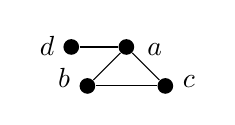
\begin{tikzpicture}[node distance=7mm,every node/.style={fill,circle,inner sep=2pt}]
\node (a) [label={[text height=1.5ex,yshift=0.0cm,xshift=0.05cm]left:$d$}] {};
\node (b) [right of=a,label={[text height=1.5ex]right:$a$}] {};
\node (c) [below left of=b,label={[text height=1.5ex,yshift=0.09cm,xshift=0.05cm]left:$b$}] {};
\node (d) [below right of=b,label={[text height=1.5ex,yshift=0.09cm,xshift=-0.05cm]right:$c$}] {};
%
\draw (a) to (b);
%
\draw (b) to (c);
\draw (b) to (d);
\draw (c) to (d);
%
\end{tikzpicture}\hspace{1em}%
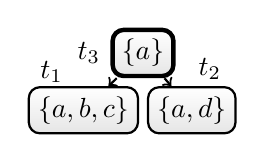
\begin{tikzpicture}[node distance=0.5mm]
%
\tikzset{every path/.style=thick}

\node (leaf1) [tdnode,label={[yshift=-0.25em,xshift=0.5em]above left:$t_1$}] {$\{a,b,c\}$};
\node (leaf2) [tdnode,label={[xshift=-1.0em, yshift=-0.15em]above right:$t_2$}, right = 0.1cm of leaf1]  {$\{a,d\}$};
\coordinate (middle) at ($ (leaf1.north east)!.5!(leaf2.north west) $);
\node (join) [tdnode,ultra thick,label={[]left:$t_3$}, above  = 1mm of middle] {$\{a\}$};

\coordinate (top) at ($ (join.north east)+(3.5em,0) $);
\coordinate (bot) at ($ (top)+(0,-4em) $);

%
\draw [->] (join) to (leaf1);
\draw [->] (join) to (leaf2);
\end{tikzpicture}%
\caption{Graph~$G$ %from Example~\ref{ex:running0}
  (left) with a TD~${\cal T}$ of graph~$G$
  (right).}%
\label{fig:graph-td}%
\end{figure}


A \emph{tree decomposition (TD)} of a given graph~$G$ is a pair
$\TTT=(T,\chi)$ where $T$ is a rooted tree and $\chi$ is a mapping
which assigns to each node $t\in V(T)$ a set~$\chi(t)\subseteq V(G)$,
called \emph{bag}, such that (i) $V(G)=\bigcup_{t\in V(T)}\chi(t)$
and
$E(G)\subseteq\SB \{u,v\} \SM t\in V(T), \{u,v\}\subseteq \chi(t)\SE$;
and (ii) for each $r, s, t\in V(T)$, such that $s$ lies on the path
from~$r$ to $t$, we have $\chi(r) \cap \chi(t) \subseteq \chi(s)$. We
let $\width(\TTT) \eqdef \max_{t\in V(T)}\Card{\chi(t)}-1$.
%
The
\emph{treewidth} $\tw(G)$ of $G$ is the minimum $\width({\TTT})$ over
all TDs~$\TTT$ of $G$.
%
For a node~$t \in V(T)$, we say that $\type(t)$ is $\leaf$ if $t$ has
no children and~$\chi(t)=\emptyset$; $\join$ if $t$ has children~$t'$ and $t''$ with
$t'\neq t''$ and $\chi(t) = \chi(t') = \chi(t'')$; $\intr$
(``introduce'') if $t$ has a single child~$t'$,
$\chi(t') \subseteq \chi(t)$ and $|\chi(t)| = |\chi(t')| + 1$; $\rem$
(``removal'') if $t$ has a single child~$t'$,
$\chi(t') \supseteq \chi(t)$ and $|\chi(t')| = |\chi(t)| + 1$. If for
every node $t\in N$, %
$\type(t) \in \{ \leaf, \join, \intr, \rem\}$, then the TD is called \emph{nice}.

\begin{example}
Figure~\ref{fig:graph-td} depicts a graph~$G$
and a TD~$\TTT$ of~$G$ of width~$2$.
  The treewidth of~$G$ is also~$2$ since~$G$ contains~\cite{Kloks94a} a complete graph with~$3$ vertices.
 % are depicted in
 % Figure~\ref{fig:graph-td}. 
\end{example}
%
%
%
%
%The formula~$F_{\leq s}$ denotes the union over all~$F_t$ for all
%descendant nodes~$t\in V(T)$ of~$s$. In other words, $F_{\leq s}$ is
%the sub-formula of~$F$ that contains all clauses that have been
%entirely covered by a bag~$\chi(s)$ for $t$ and any of its descendant
%nodes.
%

\paragraph*{Relational Algebra.}%
We use relational algebra~\cite{Codd70} for manipulation of relations,
which forms the theoretical basis of its the well-known implementation database standard 
\emph{Structured Query Language (SQL)}~\cite{} on tables.
\todo{mh: db master ref}
An \emph{attribute}~$a$ is of a certain finite \emph{domain~$\dom(a)$}.
Then, a \emph{tuple}~$r$ over set~$\attr(r)$ of attributes,
is a set of pairs of the form~$(a, v)$ with~$a\in\attr(r),v\in \dom(a)$ s.t.\ for each~$a\in \attr(r)$, there is exactly one~$v\in\dom(a)$ with~$(a,v)\in r$.
A \emph{relation~$R$} is a finite set of tuples~$r$ over set~$\attr(R)\eqdef\attr(r)$ of attributes.
Given a relation~$R$ over~$\attr(R)$.
Then, we let~$\dom(R)\eqdef \bigcup_{a\in \attr(R)}\dom(a)$, and let relation~$R$ \emph{projected to~$A\subseteq \attr(R)$} be given by $\Pi_{A}(R)\eqdef \{r_A \mid r\in R\}$, where~$r_A \eqdef \{(a, v) \mid (a, v) \in r, a \in A\}$.
This concept can be lifted to \emph{extended projection~$\dot\Pi_{A,S}$}, where we assume in addition to~$A\subseteq \attr(R)$, a set~$S$ of expressions of the form~$a \leftarrow f$, such that $a\in \attr(R)\setminus A$, and $f$ is an arithmetic function that takes a tuple~$r\in R$,
such that there is at most one expression in~$S$ for each $a\in \attr(R)\setminus A$.
Formally, we define $\dot\Pi_{A,S}(R)\eqdef \{r_A \cup r^S \mid r\in R\}$ with~$r^S \eqdef \{(a, f(r)) \mid a \in \attr(r), (a \leftarrow f) \in S\}$.
%This can be lifted to \emph{extended projection~$\dot\Pi_{E}(R)$}, where
Later, we use \emph{aggregation by grouping~$_A G_{(a\leftarrow g)}$}, where we assume~$A\subseteq \attr(R), a\in\attr(R)\setminus A$ and a so-called \emph{aggregate function~$g$}, which takes a relation~$R'\subseteq R$ and returns a value of domain~$\dom(a)$. Therefore, we let~$_A G_{(a\leftarrow g)}(R)\eqdef \{r\cup \{(a,g(R[r]))\} \mid r\in\Pi_{A}(R)\}$, where $R[r]\eqdef\{r'\mid r'\in R, r\subseteq r'\}$.
We define \emph{renaming} of~$R$ given set~$A$ of attributes, and a bijective mapping~$m:\attr(R) \rightarrow A$ s.t.\ $\dom(a)=\dom(m(a))$ for~$a\in\attr(R)$, by~$\rho_m(R) \eqdef \{(m(a),v) \mid (a,v)\in R\}$.
\emph{Selection} of rows in $R$ according to a given Boolean formula~$\varphi$ with equality\footnote{We allow for~$\varphi$ to contain expressions~$v{\approx}v'$ as variables for $v,v'\in\dom(R)\cup\attr(R)$, and we abbreviate for $v\in\attr(R)$ with~$\dom(v)=\{0,1\}$, $v{\approx}1$ by~$v$ and~$v{\approx}0$ by~$\neg v$.} is defined by~$\sigma_{\varphi}(R)\eqdef \{ r \mid r\in R, \varphi(r^E)=\emptyset \}$, where~$r^{E}$ is a truth assignment over~$\var(\varphi)$ such that for each~$v,v',v''\in\dom(R)\cup\attr(R)$ (1) $r^E(v{\approx}v')=1$ if $(v, v')\in r$, (2) $r^E(v{\approx}v)=1$, (3) $r^E(v{\approx}v')=r^E(v'{\approx}v)$, and (4) if $r^E(v{\approx}v')=1$, and $r^E(v'{\approx}v'')=1$, then $r^E(v{\approx}v'')=1$.
Given a relation~$R'$ with~$\attr(R')\cap\attr(R)=\emptyset$. Then, we refer to the \emph{cross-join} by~$R\times R'\eqdef \{ r\cup r' \mid r\in R, r'\in R'\}$.
Further, wet let \emph{$\theta$-join} correspond to~$R \bowtie_\varphi R' \eqdef \sigma_\varphi(R\times R')$.


\section{Towards Relational Algebra for Dynamic Programming}
A solver based on \emph{dynamic programming (DP)} %for formulas
evaluates the input~$\mathcal{I}$ in parts along a given TD of a graph representation~$G$
of the input.
%primal graph~$P_F$.  
Thereby, for each node~$t$ of the TD, intermediate results are %usually
stored in a \emph{table}~$\tab{t}$. %
This is achieved by running a so-called \emph{table algorithm}~$\algo{A}$,
which is designed for a certain graph representation, 
and stores in~$\tab{t}$ results of problem parts of~$\mathcal{I}$,
thereby considering tables~$\tab{t'}$ for child nodes~$t'$ of~$t$. %solves for each node~$t$ 
%
The DP approach works for many problems~$\mathcal{P}$ as follows. %proceeds in four steps.
\begin{enumerate}%
\item Construct a graph representation~$G$ of the given input instance~$\mathcal{I}$.
\item Heuristically compute a tree decomposition~$\TTT=(T,\chi)$ of~$G$.
\item\label{step:dp} Traverse the nodes in~$V(T)$ in
  post-order, i.e., perform a bottom-up traversal of~$T$.
  At every node~$t$ during post-order traversal, execute a table algorithm~$\algo{A}$ 
  that takes as input $t$, bag $\chi(t)$, a \emph{local problem}~$\mathcal{P}(t,\mathcal{I})=\mathcal{I}_t$ depending on~$\mathcal{P}$, as well as previously computed child tables of~$t$ and stores the result in~$\tab{t}$.
  %, which in turn is used by the table algorithm at
  %the parent (if exists). 
\item Interpret table~$\tab{n}$ for the root~$n$ of~$T$ in order to output the solution of~$\mathcal{I}$.
\end{enumerate}

\begin{algorithm}[t]
%\centering
  \KwData{Node~$t$, bag $\chi(t)$, clauses~$\varphi_t$,
    sequence $\langle \tab{1},\ldots \tab{\ell}\rangle$ of child tables.{~\bf Out:} Table~$\tab{t}.\hspace{-5em}$} \lIf(\hspace{-1em})
   %
  {$\type(t) = \leaf$}{%
    $\tab{t} \eqdef \{ \langle
    \tuplecolor{\specialPredColor}{\emptyset},
    \tuplecolor{\statePredColor}{1} \rangle \}$%
  }%
  \uElseIf{$\type(t) = \intr$, and
    $a\hspace{-0.1em}\in\hspace{-0.1em}\chi(t)$ is introduced}{ %
    \makebox[3.3cm][l]{$\tab{t} \eqdef \{ \langle
      \tuplecolor{\specialPredColor}{J},
      \tuplecolor{\statePredColor}{c} \rangle$
       %
    }%
    $|\;\langle \tuplecolor{\specialPredColor}{I},
    \tuplecolor{\statePredColor}{c} \rangle \in \tab{1}, \tuplecolor{\specialPredColor}{J \in \{\MAIR{I}{a\mapsto 0}, \MAIR{I}{a\mapsto 1}\}},
    \varphi_t(\tuplecolor{\specialPredColor}{J})=\emptyset\}\hspace{-5em}$\vspace{-0.05em}
       % 
  }\vspace{-0.05em}%
  % \alpha \setminus \{e \mapsto 0, e \mapsto 1\}
  \uElseIf{$\type(t) = \rem$, and $a \not\in \chi(t)$ is removed}{%
    \makebox[5.425cm][l]{$\tab{t} \eqdef \{ \langle
      \tuplecolor{\specialPredColor}{\MAR{I}},
      \tuplecolor{\statePredColor}{\Sigma_{\langle {J}, {c}\rangle
          \in \tab{1}: \MAR{I} = \MAR{J}}{c}}
      \rangle$}$|\;\langle \tuplecolor{\specialPredColor}{I},
    \tuplecolor{\statePredColor}{\cdot} \rangle \in \tab{1}
    \}\hspace{-5em}$ \vspace{-0.1em}
     %
  } %
  \uElseIf{$\type(t) = \join$}{%
    \makebox[3.3cm][l]{$\tab{t} \eqdef \{ \langle
      \tuplecolor{\specialPredColor}{I},
      \tuplecolor{\statePredColor}{c_1 \cdot c_2}
      \rangle$}$|\;\langle \tuplecolor{\specialPredColor}{I},
    \tuplecolor{\statePredColor}{c_1} \rangle \in \tab{1}, \langle
    \tuplecolor{\specialPredColor}{I},
    \tuplecolor{\statePredColor}{c_2} \rangle \in \tab{2}
    \}\hspace{-5em}$
    % 
    \vspace{-0.1em}
    % 
  } %
  %\Return $\tab{t}$ \vspace{-0.25em}
  \caption{Table algorithm~$\algo{S}(t,\chi(t),\varphi_t,\langle \tab{1}, \ldots, \tab{\ell}\rangle)$ for \cSAT~\cite{SamerSzeider10b} using nice~TD.}
  \label{alg:prim}
  \algorithmfootnote{%
    \renewcommand{\eqdef}{{\ensuremath{\,\mathrel{\mathop:}=}}}
    \label{foot:sigma}\label{foot:abrevtwo}
    %\vspace{-0.3em}
    $\MARR{S}{e} \eqdef S \setminus \{e \mapsto 0, e \mapsto
    1\}$, $\MAIR{S}{s} \eqdef S \cup \{s\}$.
    %\vspace{-1em}
    % 
  }%
\end{algorithm}%


\begin{figure}[t]
%\centering
\hspace{-0.5em}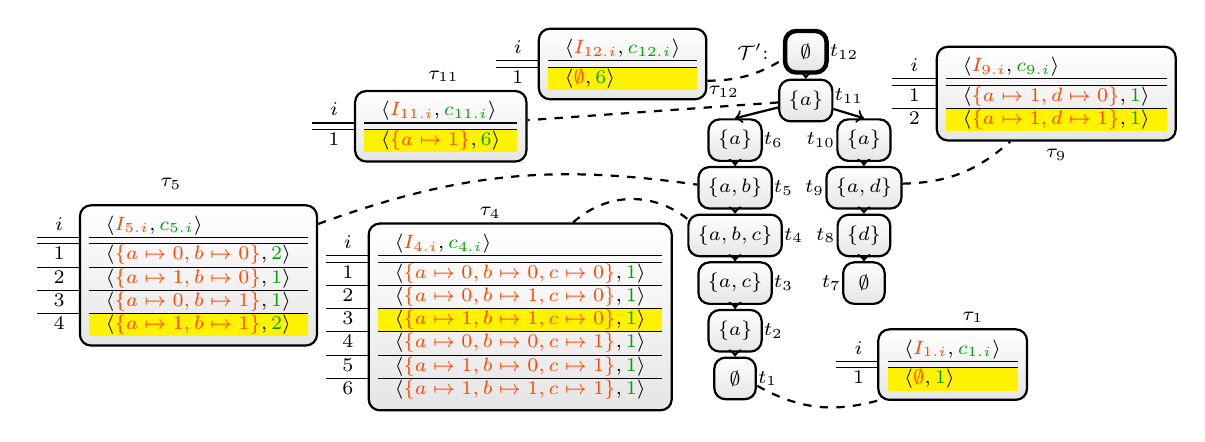
\begin{tikzpicture}[node distance=0.5mm]
%
\tikzset{every path/.style=thick}

%
\node (l1) [stdnode,label={[tdlabel, xshift=0em,yshift=+0em]right:${t_1}$}]{$\emptyset$};
\node (i1) [stdnode, above=of l1, label={[tdlabel, xshift=0em,yshift=+0em]right:${t_2}$}]{$\{a\}$};
\node (i12) [stdnode, above=of i1, label={[tdlabel, xshift=0em,yshift=+0em]right:${t_3}$}]{$\{a,c\}$};
\node (i13) [stdnode, above=of i12, label={[tdlabel, xshift=0em,yshift=+0em]right:${t_4}$}]{$\{a,b,c\}$};
\node (r1) [stdnode, above=of i13, label={[tdlabel, xshift=0em,yshift=+0em]right:${t_5}$}]{$\{a,b\}$};
\node (r12) [stdnode, above=of r1, label={[tdlabel, xshift=0em,yshift=+0em]right:${t_6}$}]{$\{a\}$};
\node (l2) [stdnode, right=2.5em of i12, label={[tdlabel, xshift=0em,yshift=+0em]left:${t_7}$}]{$\emptyset$};
\node (i2) [stdnode, above=of l2, label={[tdlabel, xshift=0em,yshift=+0em]left:${t_8}$}]{$\{d\}$};
\node (i22) [stdnode, above=of i2, label={[tdlabel, xshift=0em,yshift=+0em]left:${t_9}$}]{$\{a,d\}$};
\node (r2) [stdnode, above=of i22, label={[tdlabel, xshift=0em,yshift=+0em]left:${t_{10}}$}]{$\{a\}$};
\node (j) [stdnode, above left=of r2, yshift=-0.25em, label={[tdlabel, xshift=0em,yshift=+0.15em]right:${t_{11}}$}]{$\{a\}$};
\node (rt) [stdnode,ultra thick, above=of j, label={[tdlabel, xshift=0em,yshift=+0em]right:${t_{12}}$}]{$\emptyset$};
\node (label) [font=\scriptsize,left=of rt]{${\cal T}'$:};
%
\node (leaf1) [stdnode, left=1.25em of i1, yshift=0.5em, label={[tdlabel, xshift=2.75em,yshift=+.1em]above left:$\tab{4}$}]{%
	\begin{tabular}{l}%
		\multicolumn{1}{l}{$\langle \tuplecolor{\inputPredColor}{I_{4.i}}, \tuplecolor{\statePredColor}{c_{4.i}} \rangle$}\\
		%
		\hline\hline
		$\langle \tuplecolor{\inputPredColor}{\{a\mapsto 0, b\mapsto 0, c\mapsto 0\}}, \tuplecolor{\statePredColor}{1}\rangle$\\\hline
		$\langle \tuplecolor{\inputPredColor}{\{a\mapsto 0, b\mapsto 1, c\mapsto 0\}}, \tuplecolor{\statePredColor}{1}\rangle$\\\hline
		\rowcolor{yellow}$\langle\tuplecolor{\inputPredColor}{\{a\mapsto 1,b\mapsto 1, c\mapsto 0\}}, \tuplecolor{\statePredColor}{1}\rangle$\\\hline
		$\langle \tuplecolor{\inputPredColor}{\{a\mapsto 0, b\mapsto 0, c\mapsto 1\}}, \tuplecolor{\statePredColor}{1}\rangle$\\\hline
		$\langle\tuplecolor{\inputPredColor}{\{a\mapsto 1,b\mapsto 0,c\mapsto 1\}}, \tuplecolor{\statePredColor}{1}\rangle$\\\hline
		$\langle\tuplecolor{\inputPredColor}{\{a\mapsto 1,b\mapsto 1,c\mapsto 1\}}, \tuplecolor{\statePredColor}{1}\rangle$\\
	\end{tabular}%
};
\node (leaf1b) [stdnodenum,left=of leaf1,xshift=0.6em,yshift=0pt]{%
	\begin{tabular}{c}%
		\multirow{1}{*}{$i$}\\ %
		%
		\hline\hline
		$1$ \\\hline
		$2$ \\\hline
		$3$ \\\hline
		$4$ \\\hline
		$5$ \\\hline
		$6$
	\end{tabular}%
};
\node (leaf0x) [stdnode, left=-0.1em of leaf1b, yshift=1.5em, label={[tdlabel, xshift=2em,yshift=+.5em]above left:$\tab{5}$}]{%
	\begin{tabular}{l}%
		\multicolumn{1}{l}{$\langle \tuplecolor{\inputPredColor}{I_{5.i}}, \tuplecolor{\statePredColor}{c_{5.i}} \rangle$}\\
		%
		\hline\hline
		$\langle \tuplecolor{\inputPredColor}{\{a\mapsto 0, b\mapsto 0\}}, \tuplecolor{\statePredColor}{2}\rangle$\\\hline
		%
		$\langle\tuplecolor{\inputPredColor}{\{a\mapsto 1, b\mapsto 0\}}, \tuplecolor{\statePredColor}{1}\rangle$\\\hline
		$\langle\tuplecolor{\inputPredColor}{\{a\mapsto 0,b\mapsto 1\}}, \tuplecolor{\statePredColor}{1}\rangle$\\\hline
		\rowcolor{yellow}$\langle\tuplecolor{\inputPredColor}{\{a\mapsto 1,b\mapsto 1\}}, \tuplecolor{\statePredColor}{2}\rangle$\\
	\end{tabular}%
};
\node (leaf0b) [stdnodenum,left=of leaf0x,xshift=0.6em,yshift=0pt]{%
	\begin{tabular}{c}%
		\multirow{1}{*}{$i$}\\ %
		%
		\hline\hline
		$1$ \\\hline
		$2$ \\\hline
		$3$ \\\hline
		$4$ %
	\end{tabular}%
};
\node (leaf2b) [stdnodenum,right=2.5em of j,xshift=-0.75em,yshift=+0.25em]  {%
	\begin{tabular}{c}%
		\multirow{1}{*}{$i$}\\ %
		%
		\hline\hline
		$1$\\\hline
		$2$\\%\hline
		%
	\end{tabular}%
};
\node (leaf2) [stdnode,right=-0.4em of leaf2b, label={[tdlabel, xshift=0em,yshift=-0.25em]below:$\tab{9}$}]  {%
	\begin{tabular}{l}%
		\multirow{1}{*}{$\langle \tuplecolor{\inputPredColor}{I_{9.i}}, \tuplecolor{\statePredColor}{c_{9.i}} \rangle$}\\ %
		%
		\hline\hline
		$\langle \tuplecolor{\inputPredColor}{\{a\mapsto 1, d\mapsto 0\}}, \tuplecolor{\statePredColor}{1}\rangle$\\\hline
		%
		\rowcolor{yellow}$\langle \tuplecolor{\inputPredColor}{\{a\mapsto 1,d\mapsto 1\}}, \tuplecolor{\statePredColor}{1}\rangle$\\
	\end{tabular}%
};
\coordinate (middle) at ($ (leaf1.north east)!.5!(leaf2.north west) $);
\node (join) [stdnode,left=6.5em of r12, yshift=0.5em, label={[tdlabel, xshift=2em,yshift=+0.25em]above left:$\tab{{11}}$}] {%
	\begin{tabular}{l}%
		\multirow{1}{*}{$\langle \tuplecolor{\inputPredColor}{I_{11.i}}, \tuplecolor{\statePredColor}{c_{11.i}} \rangle$}\\
		\hline\hline
		%
		%
		%
		\rowcolor{yellow}$\langle \tuplecolor{\inputPredColor}{\{a\mapsto 1\}}, \tuplecolor{\statePredColor}{6} \rangle$\\
	\end{tabular}%
};
\node (joinb) [stdnodenum,left=-0.45em of join] {%
	\begin{tabular}{c}
		\multirow{1}{*}{$i$}\\
		\hline\hline
		%
		%
		%
		$1$\\
	\end{tabular}%
};
\node (rtx) [stdnode,left=0.0em of r12, yshift=2.75em, label={[tdlabel, xshift=0em,yshift=-1em]right:$\tab{{12}}$}] {%
	\begin{tabular}{l}%
		\multirow{1}{*}{$\langle \tuplecolor{\inputPredColor}{I_{12.i}}, \tuplecolor{\statePredColor}{c_{12.i}} \rangle$}\\
		\hline\hline
		%
		%
		%
		\rowcolor{yellow}$\langle \tuplecolor{\inputPredColor}{\emptyset}, \tuplecolor{\statePredColor}{6} \rangle$\\
	\end{tabular}%
};
\node (rtb) [stdnodenum,left=-0.45em of rtx] {%
	\begin{tabular}{c}
		\multirow{1}{*}{$i$}\\
		\hline\hline
		%
		%
		%
		$1$\\
	\end{tabular}%
};
\node (leaf0n) [stdnodenum,yshift=0.5em, right=2.5em of l1] {%
	\begin{tabular}{c}%
		\multirow{1}{*}{$i$}\\ %
		%
		\hline\hline
		$1$
	\end{tabular}%
};
%
\node (leaf0) [stdnode,right=-0.5em of leaf0n, label={[tdlabel, xshift=-1em,yshift=0.15em]above right:$\tab{1}$}] {%
	\begin{tabular}{l}%
		\multicolumn{1}{l}{$\langle \tuplecolor{\inputPredColor}{I_{1.i}}, \tuplecolor{\statePredColor}{c_{1.i}} \rangle$}\\
		%
		\hline\hline
		\rowcolor{yellow}$\langle \tuplecolor{\inputPredColor}{\emptyset}, \tuplecolor{\statePredColor}{1} \rangle$
	\end{tabular}%
};
\coordinate (top) at ($ (leaf2.north east)+(0.6em,-0.5em) $);
\coordinate (bot) at ($ (top)+(0,-12.9em) $);

\draw [<-] (j) to (rt);
\draw [->] (j) to ($ (r12.north)$);
%
%
\draw [->] (j) to ($ (r2.north)$);
\draw [->](r2) to (i22);
\draw [<-](i2) to (i22);
\draw [<-](l2) to (i2);
\draw [<-](l1) to (i1);
\draw [->](i12) to (i1);
\draw [->](i13) to (i12);
\draw [->](r1) to (i13);
\draw [->](r12) to (r1);

\draw [dashed, bend left=0] (j) to (join);
\draw [dashed, bend right=15] (rtx) to (rt);
\draw [dashed, bend right=20] (i22) to (leaf2);
\draw [dashed, bend right=40] (i13) to (leaf1);
%
\draw [dashed, bend left=22] (leaf0) to (l1);
\draw [dashed, bend left=14] (leaf0x) to (r1);
%
%
\end{tikzpicture}
\caption{Selected tables obtained by DP on~${\cal T}'$ for~$\varphi$ of Example~\ref{ex:running0} using algorithm~\algo{S}.}
\label{fig:running1}
\end{figure}


\noindent For solving problem~$\mathcal{P}=\cSAT$, we need the following graph representation.
The \emph{primal graph}~$G_\varphi$~\cite{SamerSzeider10b} of a formula~$\varphi$
has as vertices its variables, where two variables are joined by an edge
if they occur together in a clause of~$\varphi$.
Given formula~$\varphi$, a TD~$\mathcal{T}=(T,\chi)$ of~$G_\varphi$
and a node~$t$ of $T$.
%For brevity, we refer
%by~\emph{treewidth} \emph{of} a \emph{formula} to the treewidth of its
%primal graph. 
Then, we
let local problem~$\cSAT(t, \varphi)=\varphi_t$ be $\varphi_t \eqdef \SB c \SM c \in \varphi, \var(c) \subseteq \chi(t)\SE$, which are the clauses entirely covered by~$\chi(t)$.


%
%\begin{figure*}[t]%
%  {\noindent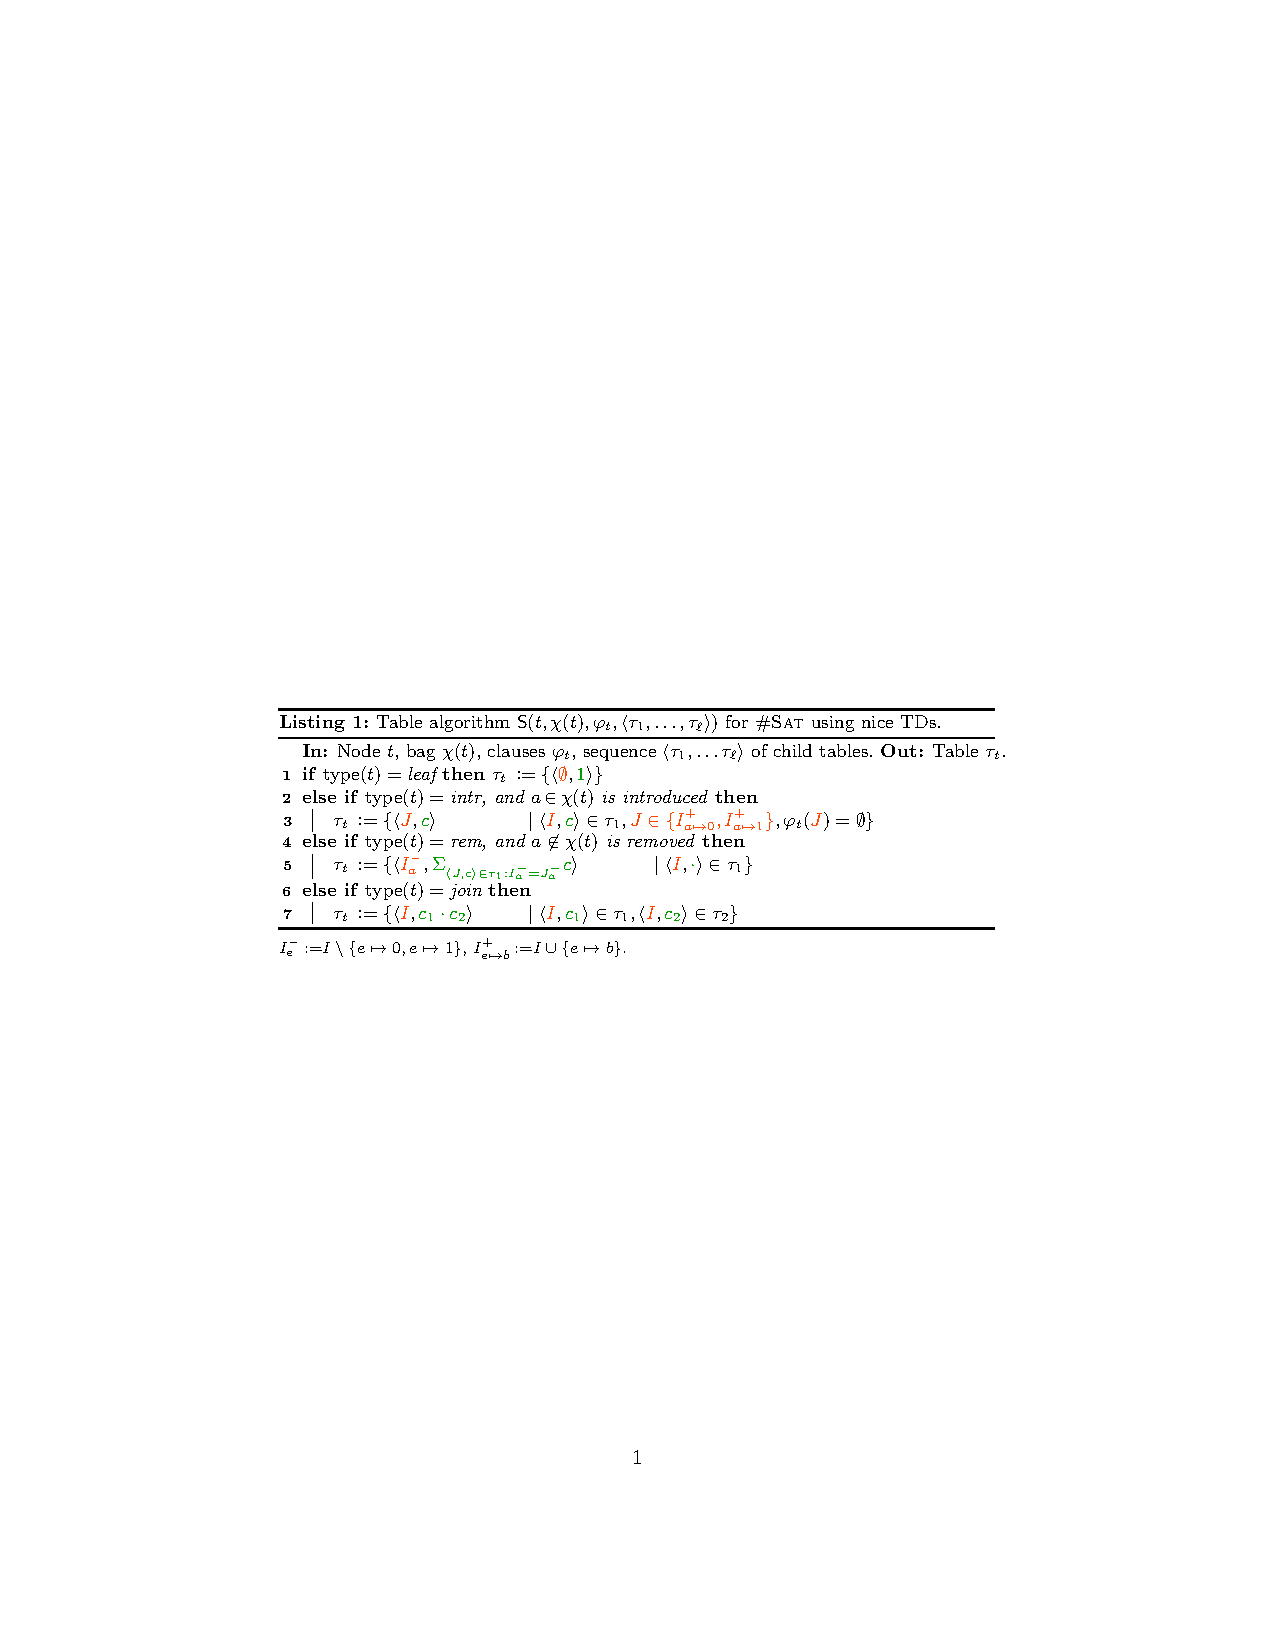
\includegraphics[trim={4.7cm 11.35cm 5cm 11.64cm},clip,page=1]{2-includes/prim.pdf}}
%%
%\end{figure*}

Table algorithm~$\algo{S}$ as presented in Listing~\ref{alg:prim} shows all the cases that are needed to solve~\cSAT by means of DP of nice TDs.
Each table~$\tab{t}$ consist of rows of the form~$\langle I, c\rangle$,
where~$I$ is an assignment of~$\varphi_t$ and~$c$ is a counter. %within a table~$\tab{t}
Nodes~$t$ with~$\type(t)=\leaf$ consist of the empty assignment and counter~$1$, cf., Line~1.
For a node~$t$ with introduced variable~$a\in\chi(t)$, we guess in Line~3 for each assignment~$\beta$ of the child table, whether~$a$ is set to true or to false, and ensure that~$\varphi_t$ is satisfied.
When an atom~$a$ is removed in node~$t$, we project assignments of child tables to~$\chi(t)$, cf., Line~5, and counters of the same assignments are summed up.
For join nodes~$t$, counters of common assignments in the child tables are multiplied as in Line~7.

\vspace{-1em}
\begin{example}\label{ex:running0}
  Consider
  formula~$\varphi\eqdef \{\overbrace{\{\neg a, b, c\}}^{c_1},
  \overbrace{\{a, \neg b, \neg c\}}^{c_2}, \overbrace{\{a,
    d\}}^{c_3}, \overbrace{\{a, \neg d\}}^{c_4}\}$.
    %
  %
  %
  Satisfying assignments of formula~$\varphi$ are, e.g., 
  $\{a\mapsto 1,b\mapsto 1, c\mapsto 0, d\mapsto 0\}$, $\{a\mapsto 1, b\mapsto 0,c\mapsto 1, d\mapsto 0\}$ or $\{a\mapsto 1, b\mapsto 1,c\mapsto 1, d\mapsto 1\}$.
  %
  %
  %
  In total, there are 6 satisfying assignments of~$\varphi$. 
  %
  %
%
%
%
%
%
%
  %
  %
  Observe that graph~$G$ of Figure~\ref{fig:graph-td} actually depicts
  the primal graph~$G_\varphi$ of~$\varphi$.
  %The primal graph~$G_\varphi$ of formula~$F$ and a tree
  %decomposition~$\TTT$ of~$G_\varphi$ are depicted in
  %Figure~\ref{fig:graph-td}. 
  Intuitively, ${\cal T}$ of Figure~\ref{fig:graph-td} allows to
  evaluate formula~$\varphi$ in parts. 
  %When evaluating $F_{\leq t_3}$, we
  %split into $F_{\leq t_1}=\{c_1,c_2\}$ and
  %$F_{\leq t_2}=\{c_3, c_4\}$, respectively.
%
%
%
%
%
  %
%
  %
  Figure~\ref{fig:running1} illustrates a nice TD~$\TTT'=(\cdot, \chi)$ of the 
  primal graph~$G_\varphi$ and
  tables~$\tab{1}$, $\ldots$, $\tab{12}$ that are obtained during the
  execution of~${\algo{S}}$ on nodes~$t_1,\ldots,t_{12}$.
  %
  %
  We assume that each row in a table $\tab{t}$ is identified by a
  number,~i.e., row $i$ corresponds to
  $\vec{u_{t.i}} = \langle I_{t.i}, c_{t.i} \rangle$.

  %
  Table~$\tab{1}=\SB \langle\emptyset, 1\rangle \SE$ as
  $\type(t_1) = \leaf$.
  %
  Since $\type(t_2) = \intr$, we construct table~$\tab{2}$
  from~$\tab{1}$ by taking~$I_{1.i}\cup\{a\mapsto 0\}$ and $I_{1.i}\cup \{a \mapsto 1\}$ for
  each~$\langle I_{1.i}, c_{1.i}\rangle \in \tab{1}$. Then,
  $t_3$ introduces $c$ and $t_4$ introduces $b$.
  $\varphi_{t_1}=\varphi_{t_2}=\varphi_{t_3} = \emptyset$, but since
  $\chi(t_4) \subseteq \var(c_1)$ we have
  $\varphi_{t_4} = \{c_1,c_2\}$ for $t_4$.
  %
  %
  %
  In consequence, for each~$I_{4.i}$ of table~$\tab{4}$, we have
  $\{c_1,c_2\}({{I_{4.i}}})=\emptyset$ since \algo{S} enforces
  satisfiability of $\varphi_t$ in node~$t$.  
  %
  %
  Since $\type(t_5) = \rem$, we remove variable~$c$ from all
  elements in $\tab{4}$ and sum up counters accordingly to construct $\tab{5}$. 
  Note that we have
  already seen all rules where $c$ occurs and hence $c$ can no
  longer affect interpretations during the remaining traversal. We
  similarly create $\tab{6}=\{\langle \{a\mapsto 0\}, 3 \rangle, \langle \{a \mapsto 1\}, 3 \rangle\}$
  and~$\tab{{10}}=\{\langle \{a \mapsto 1\}, 2 \rangle\}$.
  %
  Since $\type(t_{11})=\join$, we build table~$\tab{11}$ by taking
  the intersection of $\tab{6}$ and $\tab{{10}}$. Intuitively, this
  combines assignments agreeing on~$a$, where counters are multiplied accordingly.
  %
  %
  %
  By definition (primal graph and TDs), for every~$c \in \varphi$,
  variables~$\var(c)$ occur together in at least one common bag.
  %
  Hence, %$\varphi=\Ft{t_{12}}$ and 
  since
  $\tab{12} = \{\langle \emptyset, 6 \rangle \}$, we can reconstruct for example
  model~$\{a\mapsto 1,b \mapsto 1, c\mapsto 0, d\mapsto 1\} = I_{11.1} \cup I_{5.4} \cup I_{9.2}$ of~$\varphi$ using highlighted (yellow) rows in Figure~\ref{fig:running1}.
  On the other hand, if~$\varphi$ was unsatisfiable, $\tab{12}$ would be empty ($\emptyset$). %
  %
  %
  %
%
%
%
\end{example}%


\begin{algorithm}[t]
%\centering
  \KwData{Node~$t$, bag $\chi(t)$, clauses~$\varphi_t$,
    sequence $\langle \tab{1},\ldots \tab{\ell}\rangle$ of child tables.{~\bf Out:} Table $\tab{t}.\hspace{-5em}$} \lIf(\hspace{-1em})
   %
  {$\type(t) = \leaf$}{%
    $\tab{t} \eqdef \tuplecolor{\inputPredColor}{\{ \{{(\text{cnt}, 1)}\} \}}$ \label{line:leaf}%
  }%
  \uElseIf{$\type(t) = \intr$, and
    $a\hspace{-0.1em}\in\hspace{-0.1em}\chi(t)$ is introduced}{ %
    $\tab{t}\eqdef \tab{1} \bowtie_{\tuplecolor{\inputPredColor}{\varphi_t}} \tuplecolor{\inputPredColor}{\{\{(\cid{a},0)\},\{(\cid{a},1)\}\}}$\label{line:intr}
    \hspace{-5em}\vspace{-0.05em}
       % 
  }\vspace{-0.05em}%
  % \alpha \setminus \{e \mapsto 0, e \mapsto 1\}
  \uElseIf{$\type(t) = \rem$, and $a \not\in \chi(t)$ is removed}{%
    $\tab{t} \eqdef {_{\chi(t)}G}_{\tuplecolor{\inputPredColor}{\text{cnt$\leftarrow$\ttfamily SUM}(\text{cnt})}}(\Pi_{{\attr(\tab{1})\setminus\{\cid{a}}\}}\tab{1})$\label{line:rem} \hspace{-5em} \vspace{-0.1em}
     %
  } %
  \uElseIf{$\type(t) = \join$}{%
    \makebox[3.3cm][l]{$\tab{t} \eqdef \dot\Pi_{\chi(t),\tuplecolor{\inputPredColor}{\{\text{cnt} \leftarrow \text{cnt} \cdot \text{cnt}'\}}}(\tab{1} \bowtie_{\bigwedge_{a\in\chi(t)}\cid{a}\approx \cid{a}'} \rho_{\hspace{-1.2em}\bigcup\limits_{a\in \attr(\tab{2})}\hspace{-1.2em}\{\cid{a}\mapsto \cid{a}'\}}\tab{2})$} \label{line:join} %\{ \langle
      %\tuplecolor{\inputPredColor}{I},
      %\tuplecolor{\statePredColor}{c_1 \cdot c_2}
      %\rangle
      %$}%$|\;\langle \tuplecolor{\inputPredColor}{I},
    %\tuplecolor{\statePredColor}{c_1} \rangle \in \tab{1}, \langle
    %\tuplecolor{\inputPredColor}{I},
    %\tuplecolor{\statePredColor}{c_2} \rangle \in \tab{2}
    %\}
    \hspace{-5em}%$
    % 
    \vspace{-0.1em}
    % 
  } %
  %\Return $\tab{t}$ \vspace{-0.25em}
  \caption{Alternative table algorithm~$\algo{S_{RAlg}}(t,\chi(t),\varphi_t,\langle \tab{1}, \ldots, \tab{\ell}\rangle)$ for \cSAT.}
  \label{alg:primdb}
   %\algorithmfootnote{%
   % \renewcommand{\eqdef}{{\ensuremath{\,\mathrel{\mathop:}=}}}
   % \label{foot:sigma}\label{foot:abrevtwo}
   % %\vspace{-0.3em}
   % %$\MARR{I}{e} \eqdef I \setminus \{e \mapsto 0, e \mapsto
   % %1\}$, 
   % $\MAIR{S}{s} \eqdef S \cup \{s\}$.
   % %\vspace{-1em}
   % % 
  %}%
\end{algorithm}%


\paragraph*{Alternative: Relational Algebra.}
\noindent Instead of using set theory to describe how tables are obtained during dynamic programming 
are performed, one could alternatively use relational algebra. % or equivalent.
There, tables~$\tab{t}$ for each TD node~$t$ are pictured as relations, where~$\tab{t}$ distinguishes a unique column (attribute)~$\cid{x}$ for each~$x\in\chi(t)$.
Further, there might be additional attributes required depending on the problem at hand, e.g., we need an attribute \text{cnt} for counting in~\cSAT, or an attribute for modeling costs or weights in case of optimization problems.
Listing~\ref{alg:primdb} presents a table algorithm for problem~\cSAT that is equivalent to Listing~\ref{alg:prim}, but relies on relational algebra only for computing tables.
This step from set notation to relational algebra is driven by the observation that in these table algorithms one can identify recurring patterns, and one mainly has to adjust problem-specific parts of it (highlighted by coloring in Listing~\ref{alg:prim}).
%
%
In particular, one typically derives for nodes~$t$ with~$\type(t)=\leaf$, a fresh initial table $\tab{t}$, cf., Line~\ref{line:leaf} of Listing~\ref{alg:primdb}.
Then, whenever an atom~$a$ is introduced, such algorithms often use~$\theta$-joins with a fresh initial table for the introduced variable~$a$ that represent potential values~$a$ can have. In Line~\ref{line:intr} the selection of the $\theta$-join is performed by ensuring~$\varphi_t$, corresponding to the local problem of~\cSAT.
Further, for nodes~$t$ with~$\type(t)=\rem$, these table algorithms oftentimes need projection. 
In case of Listing~\ref{alg:primdb}, Line~\ref{line:rem} also needs grouping in order to maintain the counter, as several rows of~$\tab{1}$ might collapse in~$\tab{t}$.
Finally, for a node~$t$ with~$\type(t)=\join$, in Line~\ref{line:join} we use again $\theta$-joins (and extended projection for maintaining counters), which allows us later to leverage database technology of the last decades.

\begin{figure*}[t]%
\centering
  {\noindent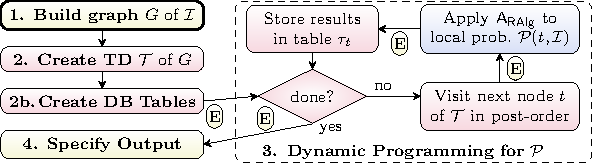
\includegraphics[]{1-figs/figure.pdf}}
  \caption{Architecture of Dynamic Programming with Databases. Steps highlighted in red are provided by the system depending on specification of yellow and blue parts, which is given by the user for specific problems~$\mathcal{P}$. The yellow ``E''s represent events that can be intercepted and handled by the user. 
  The blue part concentrates on table algorithm~$\algo{A_{RAlg}}$, where the user specifies how SQL code~is~generated in a modular~way.}
  \label{fig:arch}
%
\end{figure*}


\section{Dynamic Programming on TDs using Databases~\&~SQL}
%
%\begin{figure*}[t]%
%  {\noindent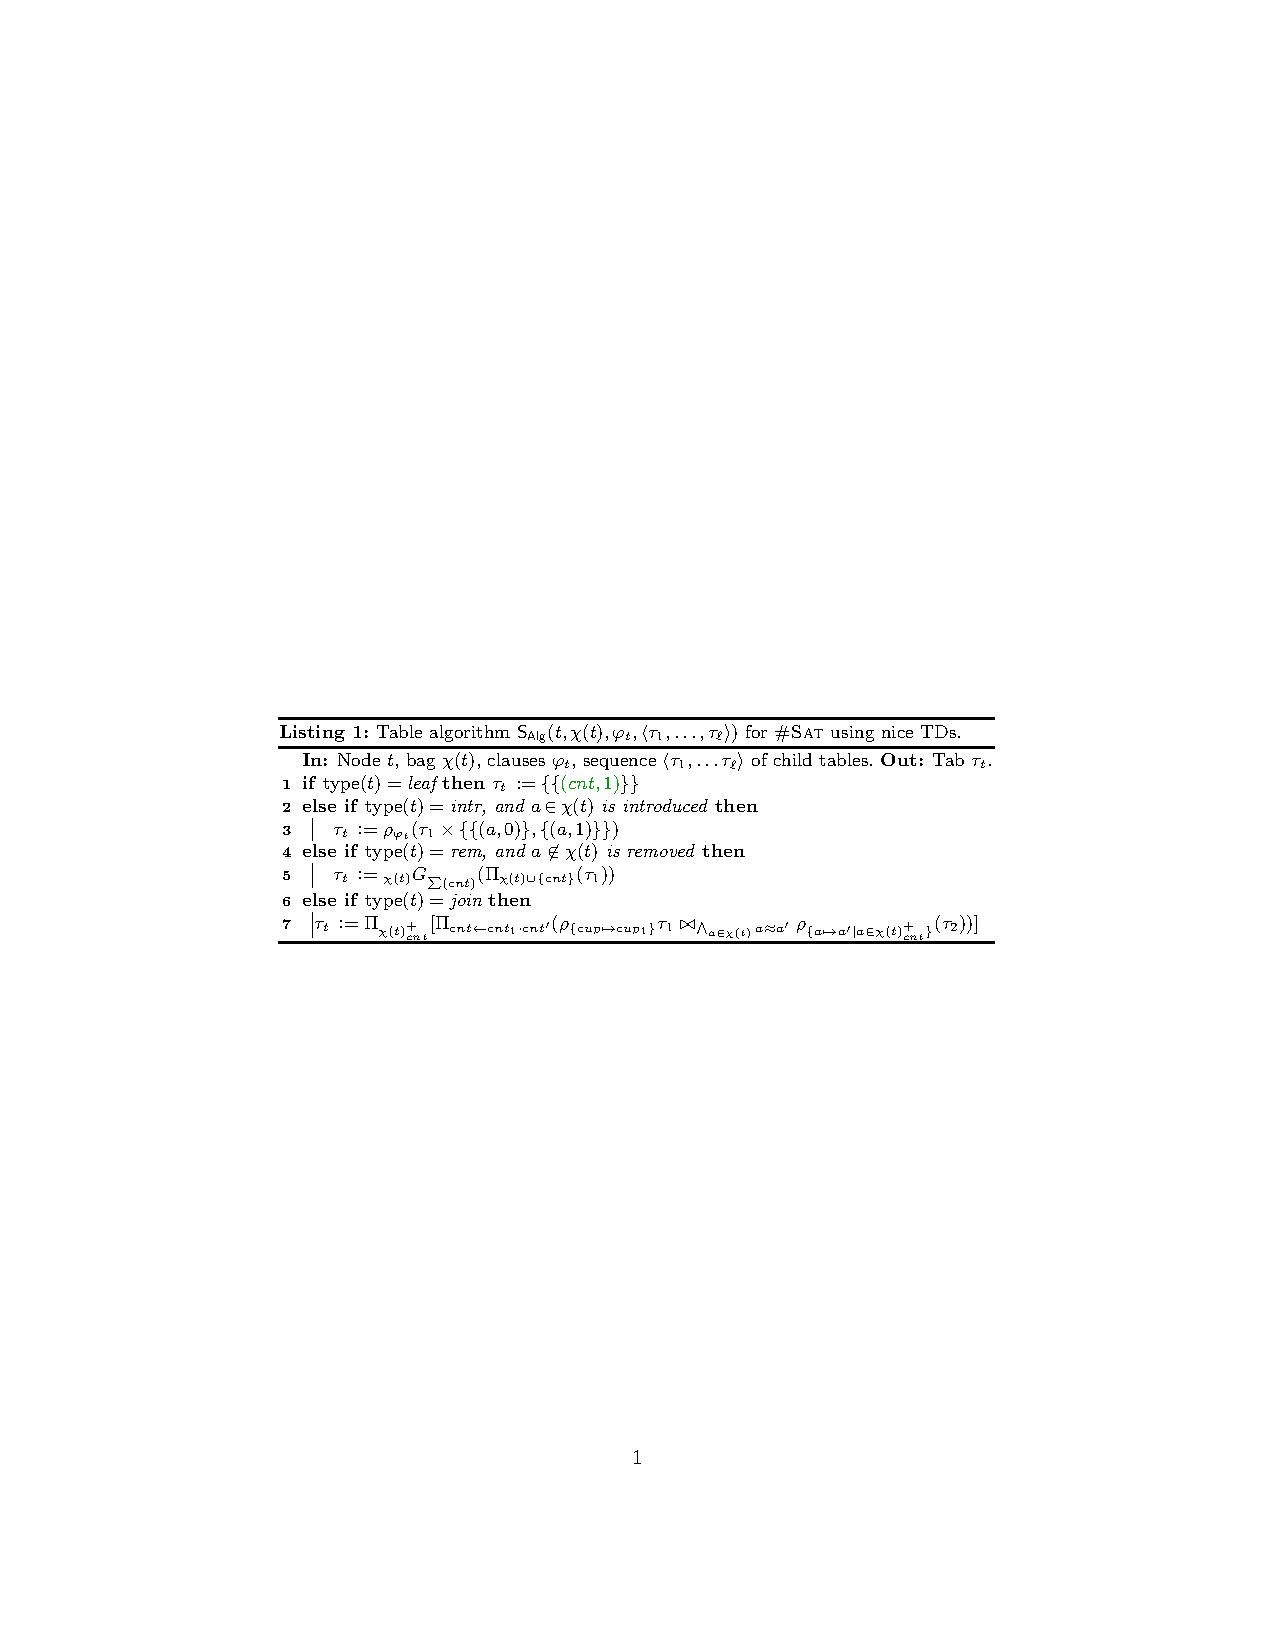
\includegraphics[trim={4.7cm 11.35cm 5cm 11.64cm},clip,page=1]{2-includes/prmdp.pdf}}
%
%\end{figure*}
%\paragraph*{Dynamic Programming on TDs.} %
%
%
In this section, we present a general architecture to model table algorithms
by means of database management systems.
The architecture is influenced by the DP approach of the previous section
and works as depicted in Figure~\ref{fig:arch},
where the steps highlighted in yellow and blue need to be specified
depending on the problem~$\mathcal{P}$. Steps outside Step~3 are mainly setup tasks,
the yellow ``E''s indicate \emph{events} that might be needed to solve more complex problems
on the polynomial hierarchy. 
For example, one could create and drop auxiliary sub-tables for each node during Step~3 within such events.
Observe that after the generation of a TD~$\mathcal{T}=(T,\chi)$, 
Step~2b automatically creates tables~$\tab{t}$ for each node~$t$ of~$T$,
where the corresponding table schema of~$\tab{t}$ is specified in the blue part, i.e., 
within~$\algo{A_{RAlg}}$. 
The \emph{default schema} of such a table~$\tab{t}$ that is assumed in this section foresees one column for each element of the bag~$\chi(t)$, where additional columns such as counters or costs can be added.

Actually, the core of this architecture is focused on the table algorithm~$\algo{A_{RAlg}}$ executed for each node~$t$ of~$T$ of TD~$\mathcal{T}=(T,\chi)$. 
Besides the definition of table schemes, the blue part concerns specification of the table algorithm by means of a procedural \emph{generator template} that describes 
how to dynamically obtain SQL code\footnote{Recall that SQL is a specific implementation standard (set) of relational algebra.} for each node~$t$ thereby oftentimes depending on~$\chi(t)$.
This generated SQL code is then used internally for manipulation of 
tables~$\tab{t}$ during the tree decomposition 
traversal in Step~3 of dynamic programming.
%
Listing~\ref{alg:template} presents a general template, where parts of table algorithms for problems that are typically problem-specific are replaced by colored placeholders of the form~$\textcolor{\inputPredColor}{\#\mathsf{placeHolder}\#}$, cf., Listing~\ref{alg:primdb}.
Note, however, that the whole architecture does not depend 
on certain normalization or forms of TDs, e.g., whether it is nice or not.
%the architecture foresees 
Instead, a table algorithm of any TD is simply specified by 
handling \emph{problem-specific} implementations of the placeholders of Listings~\ref{alg:template}, where the system following this architecture is responsible for interleaving and overlapping these cases within a node~$t$.
In fact, we discuss an implementation of a system according to this architecture next, where for efficiency it is crucial to implement non-nice TDs.

%
%
\begin{algorithm}[t]
%\centering
  \KwData{Node~$t$, bag $\chi(t)$, instance~$\mathcal{I}_t$,
    sequence $\langle \tab{1},\ldots \tab{\ell}\rangle$ of child tables.{~\bf Out:} Table $\tab{t}.\hspace{-5em}$} \lIf(\hspace{-1em})
   %
  {$\type(t) = \leaf$}{%
    $\tab{t} \eqdef \tuplecolor{\inputPredColor}{\#\epsilon\mathsf{Tab}\#}$ \label{line:leaf2}%
  }%
  \uElseIf{$\type(t) = \intr$, and
    $a\hspace{-0.1em}\in\hspace{-0.1em}\chi(t)$ is introduced}{ %
    $\tab{t}\eqdef \tab{1} \bowtie_{\tuplecolor{\inputPredColor}{\#\mathsf{localProbFilter}\#}} \tuplecolor{\inputPredColor}{\#\mathsf{intrTab}\#}$ \label{line:intr2}
    \hspace{-5em}\vspace{-0.05em}
       % 
  }\vspace{-0.05em}%
  % \alpha \setminus \{e \mapsto 0, e \mapsto 1\}
  \uElseIf{$\type(t) = \rem$, and $a \not\in \chi(t)$ is removed}{%
    $\tab{t} \eqdef {_{\chi(t)}G}_{\tuplecolor{\inputPredColor}{\#\mathsf{aggrExp}\#}}(\Pi_{\attr(\tab{1})\setminus\{\cid{a}\}}\tab{1})$ \label{line:rem2}\hspace{-5em} \vspace{-0.1em}
     %
  } %
  \uElseIf{$\type(t) = \join$}{%
    \makebox[3.3cm][l]{$\tab{t} \eqdef \dot\Pi_{\chi(t),\tuplecolor{\inputPredColor}{\#\mathsf{extProj}\#}}(\tab{1} \bowtie_{\bigwedge_{a\in\chi(t)}\cid{a}\approx \cid{a}'} \rho_{\hspace{-1.2em}\bigcup\limits_{a\in \attr(\tab{2})}\hspace{-1.2em}\{\cid{a}\mapsto \cid{a}'\}}\tab{2})$} \label{line:join2} %\{ \langle
      %\tuplecolor{\inputPredColor}{I},
      %\tuplecolor{\statePredColor}{c_1 \cdot c_2}
      %\rangle
      %$}%$|\;\langle \tuplecolor{\inputPredColor}{I},
    %\tuplecolor{\statePredColor}{c_1} \rangle \in \tab{1}, \langle
    %\tuplecolor{\inputPredColor}{I},
    %\tuplecolor{\statePredColor}{c_2} \rangle \in \tab{2}
    %\}
    \hspace{-5em}%$
    % 
    \vspace{-0.1em}
    % 
  }
  %\Return $\tab{t}$ \vspace{-0.25em}
  \caption{Template of~$\algo{A_{RAlg}}(t,\chi(t),\mathcal{I}_t,\langle \tab{1}, \ldots, \tab{\ell}\rangle)$ of Figure~\ref{fig:arch} for problem~$\mathcal{P}$.}
  \label{alg:template}
\end{algorithm}%



%\paragraph*{Problem}
%
%\begin{itemize}
%	\item events: before solve (table erstellen), after solve (table drop)
%	\item dynamic sql: introduce (table), filter (where condition), join (where inside), assignment view (for forgetting), candidate extra cols (describe how to add them)
%	\item setup: prepare input / graph, prepare tables
%	\item candidates: grundmenge
%
%\end{itemize}

\subsection{System~\dpdb: Dynamic Programming with Databases}

We implemented the proposed architecture of the previous section in the prototypical \dpdb system.
The system is open-source\footnote{Our system~\dpdb is available under GPL3 license
    at~\href{https://github.com/hmarkus/dp_on_dbs/releases/tag/TODOv1.001-pre}{\nolinkurl{github.com/hmarkus/dp_on_dbs}}.}, written in Python 3 and uses PostgreSQL as DBMS.
We are convinced though that one can easily replace PostgreSQL by any other state-of-the-art relational database that uses SQL.
%
%
In the following, we discuss implementation specifics that are crucial for a performant system that is still extendable and flexible.



\paragraph*{Computing TDs.}
TDs are computed mainly with the library \emph{htd} version~1.2 with default
settings~\cite{AbseherMusliuWoltran17a}, which finds TDs extremely quick
also for interesting instances~\cite{FichteHecherZisser19} due to heuristics.
Note that \dpdb directly supports the TD format of recent competitions,
i.e., one could easily replace the TD library.
It is crucial though to not enforce htd to compute nice TDs, as this would cause a lot of overhead later in \dpdb for copying tables.
However, in order to benefit from the implementation of $\theta$-joins,
query optimization and state-of-the-art database technology in general, 
we observed that it is crucial to limit the number of child nodes of every TD node.
Then, especially when there are huge tables involved, $\theta$-joins among child node tables
cover at most a limited number of child node tables.
In consequence, the query optimizer of the database system still has a chance
to come up with meaningful execution plans depending on the contents of the table.
Note that it is not wise though to consider $\theta$-joins which do not take into account just two tables,
since this already fixes in which order these tables shall be combined,
thereby again limiting the query optimizer.
Apart from this trade-off, we tried to outsource the task of joining tables to the DBMS as much as possible, since the performance of database systems highly depend on query optimization. % and should know best, how to join.
This actual limit, which is a restriction from experience and practice only, highly depends on the DBMS that is used.
For PostgreSQL, we set a limit of at most~$5$ child nodes for each node of the TD,
i.e., each $\theta$-join covers at most 5 child tables.

\paragraph*{Towards non-nice TDs.}
Although this paper presents the algorithms for nice TDs (mainly due to simplicity),
the system \dpdb interleaves these cases as presented in 
Listing~\ref{alg:template} automatically.
Concretely, the system executes one query per table~$\tab{t}$ for each node~$t$ during the TD traversal. 
This query consists of serveral parts and we briefly explain its parts from outside to inside. 
First of all, the inner-most part concerns the \emph{row candiates} for~$\tab{t}$ consisting of the $\theta$-join as in Line~\ref{line:join} of Listing~\ref{alg:template}, including parts of Line~\ref{line:intr}, namely cross-joins for each introduced variable, involving $\#\mathsf{intrTab}\#$ without the filtering on $\#\mathsf{localProbFilter}\#$.
Then, there are different configurations of \dpdb concerning these row candidates.
For debugging (see below) one could (1) actually materialize the result in a table,
whereas for performance runs, one should use (2) \emph{common table expressions (CTEs or {\ttfamily WITH}-queries)} or (3) \emph{subqueries (nested queries)}, which both result in one nested SQL query per table~$\tab{t}$. 
On top of these row candidates, projection\footnote{Actually, \dpdb keeps only columns relevant for the table of the parent node of~$t$.} and grouping involving~$\#\mathsf{aggrExp}\#$ as in Line~\ref{line:rem} of Listing~\ref{alg:template}, as well as selection acording to~$\#\mathsf{localProbFilter}\#$, cf., Line~\ref{line:intr}, is specified.
It turns out that PostgreSQL can do better with subqueries, where the query optimizer
oftentimes pushes selection and projection into the subquery if needed, which
is not the case for CTEs, as discussed in the PostgreSQL manual~\cite[Sec. 7.8.1]{postgres}. On different DBMS or other vendors, e.g., Oracle, it might be better to use CTEs instead.

\begin{example}\label{ex:dbviews}
Consider again Example~\ref{ex:running0} and Figure~\ref{fig:graph-td}.
If we use table algorithm~$\mathsf{S_{RAlg}}$ with \dpdb on formula~$\varphi$ of TD~$\mathcal{T}$ and Option (3): subqueries, where the row candidates are expressed via a subqueries. Then, for each node~$t_i$ of~$\mathcal{T}$, we \dpdb generates a view~$vi$ 
as well as a table~$ti$ containing in the end the content of~$vi$.
Observe that each view only has one column~$\cid{a}$ for each variable~$a$ of~$\varphi$ since the
truth assignment of the other variables are not needed later.
Actually, in \dpdb the additional columns are kept (empty, null) for readability.
This keeps the tables compact, only $t1$ has two rows, $t2$, and $t3$ have only one row.
We obtain the following views.
%
\begin{verbatim}
CREATE VIEW v1 AS SELECT a, sum(cnt) FROM 
 (WITH intrTab AS (SELECT true val UNION ALL SELECT false)
   SELECT i1.val a, i2.val b, i3.val c, 1 cnt 
          FROM intrTab i1, intrTab i2, intrTab i3)  
WHERE (NOT a OR b OR c) AND (a OR NOT b OR NOT c) GROUP BY a

CREATE VIEW v2 AS SELECT a, sum(cnt) FROM 
 (WITH intrTab AS (SELECT true val UNION ALL SELECT false) 
   SELECT i1.val a, i2.val d, 1 cnt FROM intrTab i1, intrTab i2) 
WHERE (a OR d) AND (a OR NOT d) GROUP BY a

CREATE VIEW v3 AS SELECT a, sum(cnt) FROM 
 (SELECT t1.a, t1.cnt * t2.cnt cnt FROM t1, t2 WHERE t1.a = t2.a)
GROUP BY a\end{verbatim}%
\vspace{-2em}
\end{example}%

%In other words, for each table~$\tab{t}$ of each node~$t$ of~$T$

\paragraph*{Parallelization.} A further reason to not over-restrict the number of child nodes within the TD, lies in parallelization.
In \dpdb, we compute tables in parallel along the TD,
where multiple tables can be computed at the same time,
as long as the child tables are computed.
Therefore, we tried to keep the number of child nodes in the TD as high as possible.
In our system \dpdb, we currently allow 
for at most 24 worker threads for table computations and 24 database connections at the same time (both pooled and configurable).
On top of that we have 2 additional threads and database connections for job assignments to workers, as well as one dedicated watcher thread for clean-up and termination of connections, respectively.

\paragraph*{Logging, Debugging and Extensions.} Currently, we currently have two versions of the \dpdb system implemented. 
One version aims for performance and the other one tries to achieve comprehensive logging and easy debugging of problem (instances), thereby increasing explainability.
In particular, in the latter we keep all the intermediate results, we record database timestamps before and after certain nodes, provide statistics as, e.g., width, number of rows, etc.
Further, since for each table~$\tab{t}$, exactly one SQL statement is executed for filling this table, we also have a dedicated view of the SQL {\ttfamily SELECT} statement, whose result is then inserted in~$\tab{t}$.
Together with the power and flexibility of SQL queries, we observed that this really helps in finding errors in the table algorithm specifications.

Besides convient debugging, system \dpdb immediately
contains an extension for \emph{approximation}.
There, we restrict the table contents to a maximum number of rows.
This allows for certain approximations on counting problems or
optimization problems, where it is infeasible to compute the full tables.
Further, \dpdb foresees a dedicated \emph{randomization} on these restricted number of rows
such that if one repeats the computation with a different random seed,
we obtain different approximate results.

Note that \dpdb can be easily extended. 
Each problem can overwrite existing default behavior and \dpdb also supports
problem-specific argument parser for each problem individually.
Out-of-the-box, we support the formats DIMACS CNF~\cite{}, DIMACS GRAPH~\cite{}, Edge~\cite{} as well as the format for TDs that has been used in recent competitions~\cite{}.
\todo{mh: refs!}
%sibility, 
%Supported DIMACS formats: cnf, td, tw, edge


\subsection{Table algorithms with~\dpdb for selected problems}

The system \dpdb allows for \emph{easy protyping} of DP algorithms on TDs.
This covers decision problems, counting problems as well as optimization problems.
As a proof of concept, we present the relevant parts of table algorithm specification
according to the template in Listing~\ref{alg:template}, cf., Listing~\ref{alg:primdb}.

\paragraph*{Problem~$\cSAT$.}

Specific parts for~$\cSAT$ for node~$t$ with child nodes~$t_1, \ldots, t_\ell$ and $\varphi_t = \{\{l_{1,1},\ldots,l_{1,k_1}\}, \ldots, \{l_{n,1},\ldots,l_{n,k_n}\}\}$,
where {\ttfamily ti} refers to the \emph{database table}~$\tab{i}$ for node~$t_i$ as in Example~\ref{ex:dbviews}.
\begin{itemize}
	\item\makebox[8.25em][l]{\tuplecolor{\inputPredColor}{$\#\mathsf{\epsilon Tab}\#$}:}{\ttfamily SELECT 1 AS cnt}
	\item\makebox[8.25em][l]{\tuplecolor{\inputPredColor}{$\#\mathsf{intrTab}\#$}:}{\ttfamily SELECT 1 AS val UNION ALL 0}
	\item\makebox[8.25em][l]{\tuplecolor{\inputPredColor}{$\#\mathsf{localProbFilter}\#$}:}{\ttfamily $(l_{1,1}$ OR $\ldots$ OR $l_{1,k_1})$ AND $\ldots$ AND $(l_{n,1}$ OR $\ldots$ OR $l_{n,k_n})$}
	\item\makebox[8.25em][l]{\tuplecolor{\inputPredColor}{$\#\mathsf{aggrExp}\#$}:}{\ttfamily SUM(cnt) AS cnt}
	\item\makebox[8.25em][l]{\tuplecolor{\inputPredColor}{$\#\mathsf{extProj}\#$}:}{\ttfamily t1.cnt $\cdot \ldots \cdot$ t$\ell$.cnt AS cnt }
\end{itemize}

Observe that for the corresponding decision problem~$\SAT$, where the goal is to decide only the existence of a satisfying assignment for given formula~$\varphi$, 
$\#\mathsf{epsilon Tab}\#$ returns the empty table and 
parts $\#\mathsf{aggrExp}\#, \#\mathsf{extProj}\#$ are just empty 
since there is no counter needed.


\paragraph*{Problem~$\cTCOL$.}
Given a graph~$G=(V,E)$, a \emph{$o$-coloring} is a mapping~$\iota: V \rightarrow \{1,\ldots,o\}$
such that for each edge~$\{u,v\}\in E$, we have~$\iota(u)\neq \iota(v)$.
Problem~$\cTCOL$ asks to count the number of $o$-colorings of~$G$.
Local problem~$\cTCOL(t,G)$ is defined by the graph $G_t \eqdef (V\cap\chi(t), E\cap [\chi(t)\times\chi(t)])$.

Specific parts for~$\cTCOL$ for node~$t$ with child nodes~$t_1, \ldots, t_\ell$
are as follows, where~$E(G_t)=\{\{u_1,v_1\},\ldots, \{u_n,v_n\}\}$.
%
%where {\ttfamily ti} refers to the database table~$\tab{i}$ for node~$t_i$ as in Example~\ref{ex:dbviews}.
\begin{itemize}
	\item\makebox[8.25em][l]{\tuplecolor{\inputPredColor}{$\#\mathsf{\epsilon Tab}\#$}:}{\ttfamily SELECT 1 AS cnt}
	\item\makebox[8.25em][l]{\tuplecolor{\inputPredColor}{$\#\mathsf{intrTab}\#$}:}{\ttfamily SELECT 1 AS val UNION ALL $\ldots$ UNION ALL $u$}
	%\item\makebox[6em][l]{\tuplecolor{\inputPredColor}{$\#\mathsf{localProbFilter}\#$}:}{\ttfamily \cid{u1} OR \cid{ SELECT 1 AS val UNION ALL 2 UNION ALL 3}
	\item\makebox[8.25em][l]{\tuplecolor{\inputPredColor}{$\#\mathsf{localProbFilter}\#$}:}{\ttfamily NOT $(\cid{u_1}=\cid{v_1})$ AND $\ldots$ AND NOT $(\cid{u_n}=\cid{v_n})$}
	\item\makebox[8.25em][l]{\tuplecolor{\inputPredColor}{$\#\mathsf{aggrExp}\#$}:}{\ttfamily SUM(cnt) AS cnt}
	\item\makebox[8.25em][l]{\tuplecolor{\inputPredColor}{$\#\mathsf{extProj}\#$}:}{\ttfamily t1.cnt $\cdot \ldots \cdot$ t$\ell$.cnt AS cnt }
\end{itemize}



\paragraph*{Problem~\VC.}
Given a graph~$G=(V,E)$, a \emph{vertex cover} is a set of vertices~$C\subseteq V$ of~$G$
such that for each edge~$\{u,v\}\in E$, we have~$\{u,v\}\cap C\neq \emptyset$.
Then, \VC asks to find the minimum cardinality~$|C|$ among all vertex cover~$C$, i.e., $C$ is such that there is no vertex cover~$C'$ with~$|C'| < |C|$. 
Local problem~$\VC(t,G)\eqdef G_t$ is defined as above. 
%by the graph $G_t \eqdef (V\cap\chi(t), E\cap [\chi(t)\times\chi(t)])$.
To this end, we use an additional column {\ttfamily card} for storing cardinalities.

Problem $\VC$ for node~$t$ with child nodes~$t_1, \ldots, t_\ell$, where~$E(G_t)=\{\{u_1,v_1\},\ldots, \{u_n,v_n\}\}$ can be specified as follows.

\begin{itemize}
	\item\makebox[8.25em][l]{\tuplecolor{\inputPredColor}{$\#\mathsf{\epsilon Tab}\#$}:}{\ttfamily SELECT 0 AS card}
	\item\makebox[8.25em][l]{\tuplecolor{\inputPredColor}{$\#\mathsf{intrTab}\#$}:}{\ttfamily SELECT 1 AS val UNION ALL 0}
	\item\makebox[8.25em][l]{\tuplecolor{\inputPredColor}{$\#\mathsf{localProbFilter}\#$}:}{\ttfamily $(\cid{u_1}$ OR $\cid{v_1})$ AND $\ldots$ AND $(\cid{u_n}$ OR $\cid{v_n})$}
	\item\makebox[8.25em][l]{\tuplecolor{\inputPredColor}{$\#\mathsf{aggrExp}\#$}:}{\ttfamily MIN(card) AS card}
	\item\makebox[8.25em][l]{\tuplecolor{\inputPredColor}{$\#\mathsf{extProj}\#$}:}%{\ttfamily t1.cnt $\cdot \ldots \cdot$ t$\ell$.cnt }
\end{itemize}

Similar to \VC and \cTCOL one can model several other (graph) problems.
One could also think of counting the number of solutions of problem \VC,
where both a column for cardinalities and one for counting is used. 
There, in addition to grouping with {\ttfamily GROUP BY} in \dpdb, we additionally could use the {\ttfamily HAVING} construct of SQL,
where only rows are kept, whose column {\ttfamily card} is minimal.


%#\begin{algorithm}[h]
%#  \KwData{Node~$t${~\bf Out:} SQL query}
%#  \KwRet{\{0,1\}}\;
%#  \caption{introduce}
%#  \label{alg:introduce}
%#\end{algorithm}
%#
%#\begin{algorithm}[h]
%#  \KwData{Node~$t${~\bf Out:} SQL expression}
%#  \KwRet{"sum(cnt)"}\;
%#  \caption{aggregate}
%#  \label{alg:aggregate}
%#\end{algorithm}
%#
%#\begin{algorithm}[h]
%#  \KwData{Node~$t${~\bf Out:} SQL WHERE-condition}
%#  \KwRet{$\varphi_t$}\;
%#  \caption{filter}
%#  \label{alg:filter}
%#\end{algorithm}
%#
%#\begin{algorithm}[h]
%#  \KwData{Node~$t$, sequence $\langle \tab{1},\ldots \tab{\ell}\rangle$ of child tables.{~\bf Out:} SQL expression}
%#  \KwRet{"$\tab{1}.cnt * \ldots * \tab{\ell}.cnt$"}\;
%#  \caption{extra\_projection}
%#  \label{alg:extraprojection}
%#\end{algorithm}
%#
%#\if 0
%#["{} AS model_count".format(
%#                " * ".join(set([var2cnt(node,v) for v in node.vertices] +
%#                               [node2cnt(n) for n in node.children])) if node.vertices or node.children else "1"
%#                )]
%#\fi
%#

%\paragraph*{TODO:}
%\begin{itemize}
	%\item Examples (pseudo-code) for sharpsat (and maybe min-VC)
	%\item limit result rows (+ possibly randomize) of each node for faster approximations.
	%\item approximate memory used by db for one of the largest problems solved
	%\item Supported DIMACS formats: cnf, td, tw, edge
	%\item Discussion section: we don't create/use any indices... Meaningful/useful B*Tree indices hard to create. Exploration of Bitmap indices (Oracle Enterprise feature) would be interesting.
%\end{itemize}



\section{Experiments}
\label{sec:experiments}
%
We conducted a series of experiments using publicly available benchmark sets for~\cSAT.
%model counting and weighted model counting. 
Our tested benchmarks~\cite{FichteEtAl18b} 
are publicly available,
and our results are
also on github at
\href{https://github.com/hmarkus/dp_on_dbs/tree/padl2020}{\nolinkurl{github.com/hmarkus/dp_on_dbs/padl2020}}.

\subsection{Setup}

\paragraph{Measure \& Resources.}
%As we use different types of hardware in our experiments and other
%natural measures such as power consumption cannot be recorded with
%current hardware, 
We mainly compare wall clock time and number of
timeouts. 
In the time we include, if applicable, \emph{preprocessing
  time} as well as \emph{decomposition time} for computing a %30
TD with a fixed random seed. % and decomposition selection time.
%
%However, we avoid IO access on the CPU solvers whenever possible,
%i.e., we load instances into the RAM before we start solving.
%
For parallel CPU solvers we allow access to 24 physical cores on
machines, where hyperthreading was disabled.
%
%
%
%
%
We set a timeout of 900 seconds and limited available RAM to~14 GB per
instance and solver.

\paragraph{Benchmark Instances.}
We considered a selection of overall 1494 instances from various
publicly available benchmark sets~\cSAT consisting of %
%
%
%
%
\instances{fre/meel} benchmarks\footnote{See:
  \href{http://tinyurl.com/countingbenchmarks}{\nolinkurl{tinyurl.com/countingbenchmarks}}}(1480
instances), %
and \instances{c2d} benchmarks\footnote{See:
  \href{http://reasoning.cs.ucla.edu/c2d/results.html}{\nolinkurl{reasoning.cs.ucla.edu/c2d}}}
(14 instances).
However, we used instances after being preprocessed by pmc,
similar to a recent work on~\cSAT~\cite{FichteEtAl19}
There, more than 80\% of the \cSAT instances have primal treewidth below~19
after preprocessing.
Before preprocessing
%, for which decomposer takes 0.1 seconds in median.
%
%Overall, both B+E and pmc managed to \emph{drastically reduce} the
%widths, the decomposer ran below 0.1 seconds in median.
%
%
%For~\WMC, we used the overall 1091 instances from the
%\instances{Cachet} benchmark set\footnote{See:
%  \href{https://www.cs.rochester.edu/u/kautz/Cachet/Model_Counting_Benchmarks/index.html}{\nolinkurl{cs.rochester.edu/u/kautz/Cachet}}}.
%

\paragraph{Benchmarked Solvers.}
In our experimental work, we present results for the most recent
versions of publicly available \cSAT solvers, namely,
%
\href{http://reasoning.cs.ucla.edu/c2d/download.php}{\textit{c2d}~2.20}~\cite{Darwiche04a},
\href{http://www.cril.univ-artois.fr/KC/d4.html}{\textit{d4}~1.0}~\cite{LagniezMarquis17a},
\href{https://bitbucket.org/haz/dsharp}{\textit{DSHARP}~1.0}~\cite{MuiseEtAl12a},
\href{http://reasoning.cs.ucla.edu/minic2d/}{\textit{miniC2D}~1.0.0}~\cite{OztokDarwiche15a},
\href{http://www.cril.univ-artois.fr/KC/eadt.html}{\textit{cnf2eadt}~1.0}~\cite{KoricheLagniezMarquisThomas13a}, 
\href{http://www.sd.is.uec.ac.jp/toda/code/cnf2obdd.html}{\textit{bdd\_{}minisat\_\allowbreak{}all}~1.0.2}~\cite{TodaSoh15a},
and \href{http://reasoning.cs.ucla.edu/sdd/}{\textit{sdd}~2.0}~\cite{Darwiche11a} (based on %
knowledge compilation techniques).
%
%
%
%
%
%
%
We also considered rather recent approximate solvers
\href{https://bitbucket.org/kuldeepmeel/approxmc}{\textit{ApproxMC2}, \textit{ApproxMC3}}~\cite{ChakrabortyEtAl14a}
and
\href{http://cs.stanford.edu/~ermon/code/STS.zip}{\textit{sts}~1.0}~\cite{ErmonGomesSelman12a},
%
as well as %
CDCL-based solvers
%
\href{https://www.cs.rochester.edu/u/kautz/Cachet/cachet-wmc-1-21.zip}{\textit{Cachet}~1.21}~\cite{SangEtAl04},
\href{http://tools.computational-logic.org/content/sharpCDCL.php}{\textit{sharpCDCL}}\footnote{See:
  \href{http://tools.computational-logic.
    org/content/sharpCDCL.php}{\nolinkurl{tools.computational-logic.
      org}}}, %
and
\href{https://sites.google.com/site/marcthurley/sharpsat}{\textit{sharpSAT}~13.02}~\cite{Thurley06a}.
%
Finally, we also included multi-core solvers
\href{https://github.com/daajoe/GPUSAT/releases/tag/v0.815-pre}{\textit{gpusat}~1.0 and \textit{gpusat}~2.0}~\cite{FichteEtAl19}, as well as
\textit{countAntom}~1.0~\cite{BurchardSchubertBecker15a} on 12 physical CPU
cores, which performed better than on 24 cores.
%
%
%
%
%
%
%
%
%Note that we benchmarked additional solvers, which we omitted from the
%presentation here and where we placed results online in our result
%data repository.
%%
%For~\WMC, 
We considered also additional solvers, e.g., %\textit{sts},
%\textit{\gpusatone}, \gpusatnu, \textit{miniC2D}, \textit{Cachet},
%\textit{d4}, and
\href{http://www.cril.univ-artois.fr/kc/ressources/query-dnnf-0.4.180625.zip}{\textit{d-DNNF
    reasoner}~0.4.180625} on top of d4 as underlying knowledge
compiler, where detailed results can be found online. %
All experiments were conducted with default solver options.
%
%
%For solver~\gpusatnu, we also benchmarked variant~\gpusatnuv{A+B}
%where we used 30 as threshold above which we apply the BST.
%
%
%
%
%
%
%



%\begin{figure}[bt]
%\centering
%\vspace{0pt}\includegraphics[height=13em]{plot_Width_sat.pdf}%
%%\hspace{6pt}\includegraphics[height=13em]{plot_Width_wmc.pdf}%
%\caption{%
%  Width distribution of~\cSAT instances (left) before and after
%  preprocessing (using both B+E and pmc).  Width distribution of~\WMC
%  instances (right) before and after preprocessing using pmc*.
%  Results are based on the primal treewidth and presented in
%  intervals.  X-axis labels the intervals, y-axis labels the number of
%  instances.
%%
%}%
%\label{fig:distribution}
%\end{figure}
%

\paragraph{Benchmark Hardware.}
%
%
%
%
Almost all solvers were executed on a cluster of 12 nodes. Each node is equipped
with two Intel Xeon E5-2650 CPUs consisting of 12 physical cores each
at 2.2 GHz clock speed and 256 GB RAM. %
The results were gathered on Ubuntu~16.04.1 LTS machines with disabled hyperthreading
on kernel~4.4.0-139. %, which is already a post-Spectre and
%post-Meltdown kernel\footnote{Details on spectre and meltdown: \href{https://spectreattack.com/}{\nolinkurl{spectreattack.com}}.}.
%
%
For~\gpusatone and~\gpusatnu we used a machine equipped with a consumer GPU:
%
Intel Core i3-3245 CPU operating at 3.4 GHz, 16 GB RAM, and one
Sapphire Pulse ITX Radeon RX 570 GPU running at 1.24 GHz with 32
compute units, 2048 shader units, and 4GB VRAM using driver
amdgpu-pro-18.30-641594 and OpenCL~1.2.
The system operated on Ubuntu~18.04.1 LTS with kernel 4.15.0-34.
%




%
%
%
%
%
%
%
%
%
%
%
%
%
%
%
%
%
%
%
%
%
%
%
%
%
%
%
%
%
%
%
%
%
%
%



%\begin{table}[bt]
%  \centering
%  \resizebox{\columnwidth}{!}{%
%    \begin{tabular}{{l|l|rr|rHr|rHr||rrrrr||rrrH}}
%      \toprule
%      prob & pre &  vMdn & cMdn & t[s] Mdn & t[s] Max & to & t[s] Mdn pre & t[s] Max pre & to & Mdn & 50\% & 80\% & 90\% & 95\% & min & max & mdn & mean \\
%      \midrule
%      \cSAT & w/o pre & 637 & 810 & 0.07 & 1800.0 & \textbf{6} & n/a & n/a & n/a & 31 & 31 & 166 & 378 & 922 & n/a & n/a & n/a & n/a \\
%      & pmc, B+E & \textbf{231} & 350 & 0.02 & 1800.0 & \textbf{6} & 0.06 & 900.0 & 192 & \textbf{3} & \textbf{3} & \textbf{17} & 201 & \textbf{823} & -72 & \textbf{755} & 22 & \textbf{31.9} \\
%      & pmc & \textbf{231} & 189 & 0.03 & 1800.0 & \textbf{6} & \textbf{0.03} & 900.0 & \textbf{103} & \textbf{3} & 4 & 19 & 228 & \textbf{823} & -1839 & 547 & \textbf{23} & 23.1 \\
%      & B+E & \textbf{231} & \textbf{185} & \textbf{0.02} & 1800.0 & \textbf{6} & 0.04 & 900.0 & 189 & \textbf{3} & \textbf{3} & 18 & \textbf{192} & \textbf{823} & 
%                                                                                                                                                                    \textbf{-2} & 633 & \textbf{23} & 31.7 \\
%      \midrule
%      \WMC & w/o pre & \textbf{200} & 519 & 0.04 & 9.21 & \textbf{0} & n/a & n/a & n/a & 28 & 28 & 40 & 43 & 54 & n/a & n/a & n/a & n/a \\
%           & pmc* & \textbf{200} & \textbf{300} & \textbf{0.03} & 1.6 & \textbf{0} & \textbf{0.03} & 1.6 & \textbf{0} & \textbf{11} & \textbf{11} & \textbf{20} & \textbf{25} & \textbf{30} & \textbf{0} & \textbf{330} & \textbf{16} & \textbf{18.8} \\
%      \bottomrule
%    \end{tabular}
%  }
%  \medskip
%  \caption{Overview on upper bounds of the primal treewidth for
%    considered \cSAT and \WMC benchmarks before and after
%    preprocessing.  vMdn median of variables, cMdn median of clauses,
%    t[s] Mdn of the decomposition runtime in seconds, maximum runtime
%    t[s] Max, median Mdn and percentiles of upper bounds on treewidth,
%    and min/max/mdn %
%    of the width improvement after preprocessing. Negative values
%    indicate worse results.  }
%\label{tab:tw_combined}
%  \label{tab:tw_combined_wmc}
%\label{tab:detailed}
%\end{table}
%

\subsection{Results} % \& Discussion}

%
%
%
%
%
%
%
%
%
%


\begin{figure}[t]
  %
  %
  \centering
  \resizebox{.7\columnwidth}{!}{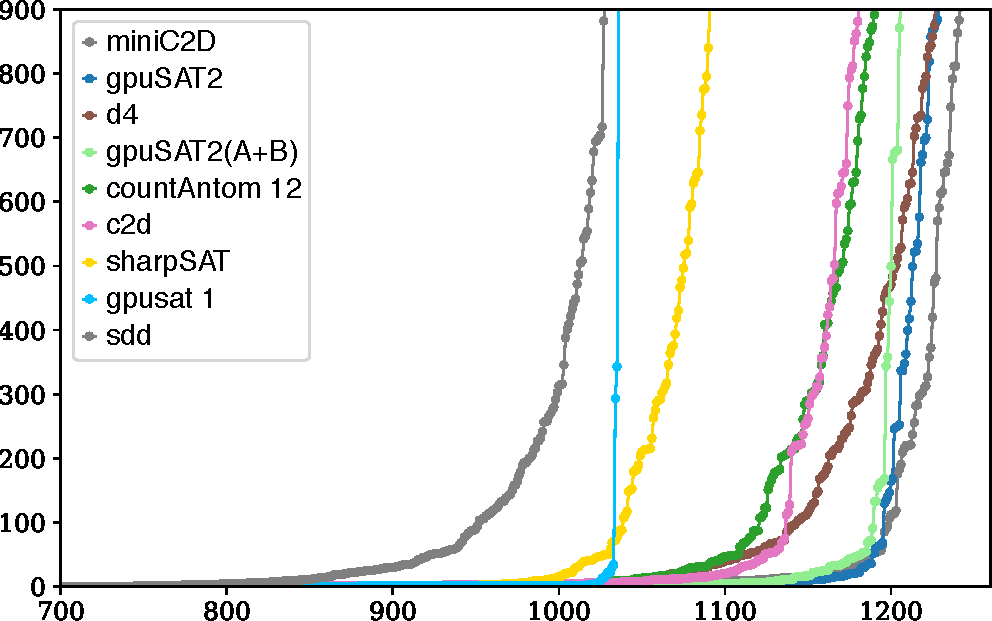
\includegraphics{plot_pmc_enlarged.pdf}}
  %
  %
  %
  %
  %
  %
  \caption{Runtime for the top 5 sequential and all parallel solvers over all the~\cSAT instances with pmc preprocessor. %
    %
    %
    The x-axis refers to the number of instances and the y-axis
    depicts the runtime sorted in ascending order for each solver
    individually.  }
  \label{fig:runtime}
\end{figure}
%
Figure~\ref{fig:runtime} illustrates the top five sequential solvers,
and all parallel counting solvers %
%
with preprocessor pmc %
%
in a cactus-like plot. 
Table~\ref{tab:sat:merged} presents detailed runtime
results for~\cSAT with preprocessors pmc, B+E, and without preprocessing, respectively.
%
%
%
%
%
%
%
%
%
%
%
%
%
%
%
%
Since the solver sts produced results that varied from the correct
result on average more than the value of the correct result, %
%
%
%
%
%
we excluded it from the presented results.  If we disallow
preprocessing, \gpusatnu and \gpusatone perform only slightly better
in the overall standing of the solvers. But \gpusatnu solves 42
instances more and requires about 10 hours less of wallclock
time. Further, we can observe, that %
the variant~\gpusatnuv{A+B} performs particular well, mainly since for
instances below width~30, the BST compression seems relatively
expensive compared to the array data structure.
%
%
%
%
%
Interestingly, when considering the results on preprocessing in
Table~\ref{tab:sat:merged} (top, mid) and Figure~\ref{fig:runtime} we
observe that the architectural improvements pay off quite
well. \gpusatnu can solve the vast majority of the instances and
ranks second place.  If one uses the B+E preprocessor shown in
Table~\ref{tab:sat:merged} (mid), \gpusatnu solves even more instances
as well as the other solvers. Still, it ranks fifth solving only 26
instances less than the best solver and 10 less than the third best
solver and solves the most instances having width below 30.

\newcommand{\inacc}[1]{\ensuremath{\diamond{}}#1}
\begin{table}[tb]
  \centering
  \resizebox{0.8\columnwidth}{!}{%
    \begin{tabular}{{l|lH||rrrrrrrr||r||rHr}}
      \toprule
      & solver & racc & 0-20 & 21-30 & 31-40 & 41-50 & 51-60 & $>$60 & best & unique & $\sum$ & time[h] & rank \\
      \midrule
      \parbox[t]{1em}{\multirow{9}{*}{\rotatebox[origin=c]{90}{pmc preprocessing}}}&miniC2D & \textbf{0} & 1193 & 29 & \textbf{10} & 2 & 1 & 7 & 13 & 0 & \textbf{1242} & \textbf{68.77} & 1 \\
      &\gpusatnu & 4.7E-15 & \textbf{1196} & 32 & 1 & 0 & 0 & 0 & 250 & %
                                                                                     \textbf{8} & 1229 & 71.27 & 2 \\
     %
      &d4 & \textbf{0} & 1163 & 20 & \textbf{10} & 2 & \textbf{4} & 28 & 52 & 1 & 1227 & 76.86 & 3 \\
      %
      & \gpusatnuv{A+B} & {4.6E-15} & {1187} & 18 & 1 & 0 & 0 & 0 & 120 & 7 & 1206 & 74.56 & 4 \\
      &countAntom 12 & \textbf{0} & 1141 & 18 & \textbf{10} & \textbf{5} & \textbf{4} & 13 & 101 & 0 & 1191 & 84.39 & 5 \\
      &c2d & \textbf{0} & 1124 & 31 & \textbf{10} & 3 & 3 & 10 & 20 & 0 & 1181 & 84.41 & 6 \\
      &sharpSAT & \textbf{0} & 1029 & 16 & \textbf{10} & 2 & \textbf{4} & \textbf{30} & \textbf{253} & 1 & 1091 & 106.88 & 7 \\
      &\gpusatone & 1.7E-13 & 1020 & 16 & 0 & 0 & 0 & 0 & 106 & 7 & 1036 & 114.86 & 8 \\
      & sdd & \textbf{0} & 1014 & 4 & 7 & 1 & 0 & 2 & 0 & 0 & 1028 & 124.23 & 9 \\
      %
      %
      \midrule
      & solver & racc & 0-20 & 21-30 & 31-40 & 41-50 & 51-60 & $>$60 & best & unique & $\sum$ & time[h] & rank \\
      \midrule
      \parbox[t]{1em}{\multirow{8}{*}{\rotatebox[origin=c]{90}{B+E preprocessing}}}&c2d & \textbf{0} & 1199 & 24 & \textbf{9} & 0 & 2 & 23 & 14 & 0 & \textbf{1257} & \textbf{63.46} & 1 \\
      &miniC2D & \textbf{0} & 1203 & \textbf{27} & 8 & 0 & 2 & 12 & 8 & 0 & 1252 & 64.92 & 2 \\
      &d4 & \textbf{0} & 1182 & 15 & \textbf{9} & \textbf{1} & \textbf{3} & 31 & 79 & 1 & 1241 & 69.32 & 3 \\
      &countAntom 12 & \textbf{0} & 1177 & 14 & 8 & 0 & 2 & \textbf{34} & 100 & 0 & 1235 & 69.79 & 4 \\
      %
      &\gpusatnu & 6.4E-16 & \textbf{1204} & 26 & 1 & 0 & 0 & 0 & \textbf{150} & \textbf{3} & 1231 & 68.15 & 5 \\
      %
      &\gpusatnuv{A+B} & {6.4E-16} & 1201 & 21 & 1 & 0 & 0 & 0 & 67 & \textbf{3} & 1223 & 70.39 & 6 \\
      &sdd & \textbf{0} & 1106 & 11 & 4 & \textbf{1} & 1 & 4 & 0 & 0 & 1127 & 100.48 & 7 \\
      &\gpusatone & 9.9E-12 & 1037 & 16 & 0 & 0 & 0 & 0 & 87 & %
                                                               \textbf{3} & 1053 & 110.87 & 8 \\
                                                               %
      &bdd\_minisat\_all & \textbf{0} & 926 & 6 & 3 & \textbf{1} & 1 & 0 & 101 & 0 & 937 & 140.59 & 9 \\
      %
      \midrule
      &solver & racc & 0-20 & 21-30 & 31-40 & 41-50 & 51-60 & $>$60 & best & unique & $\sum$ & time[h] & rank \\
      %
      \midrule
      \parbox[t]{1em}{\multirow{9}{*}{\rotatebox[origin=c]{90}{without preprocessing}}}& countAntom 12 & \textbf{0} & 118 & 511 & 139 & \textbf{175} & \textbf{21} & \textbf{181} & 318 & 15 & \textbf{1145} & \textbf{96.64} & 1 \\
      & d4 & \textbf{0} & 124 & 514 & 148 & 162 & \textbf{21} & 168 & 69 & 15 & 1137 & 104.94 & 2 \\
      & c2d & \textbf{0} & 119 & 525 & \textbf{165} & 161 & 18 & 120 & 48 & 15 & 1108 & 110.53 & 3 \\
      & miniC2D & \textbf{0} & 122 & 514 & 128 & 149 & 9 & 62 & 0 & 0 & 984 & 141.22 & 4 \\
      & sharpSAT & \textbf{0} & 100 & 467 & 124 & 156 & 12 & 123 & \textbf{390} & 4 & 982 & 135.41 & 5 \\
      %
      %
      %
      & \gpusatnuv{A+B} & {9.8E-18} & \textbf{125} & \textbf{539} & 96 & 138 & 0 & 0 & 94 
                                                                            & \textbf{19} & 898 & 151.16 & 8 \\
      %
                                                                            %
                                                                            %
                                                                            %
                                                                            %
                                                                            %
      &\gpusatnu & 9.7E-18 & \textbf{125} & 523 & 96 & 138 & 0 & 0 & 78 & 17 & 882 & 155.43 & 8 \\
      %
      &\gpusatone & 1.4E-10 & \textbf{125} & 524 & 67 & 140 & 0 & 0 & 82 & %
                                                                           9 & 856 & 162.03 & 11 \\
      &cachet & \textbf{0} & 99 & 430 & 71 & 152 & 8 & 57 & 3 & 0 & 817 & 176.26 & 12 \\
      %
      \midrule
      &solver & racc & 0-20 & 21-30 & 31-40 & 41-50 & 51-60 & $>$60 & best & unique & $\sum$ & time[h] & rank \\
      \bottomrule
    \end{tabular}
  }
  \caption{%
    Number of~\cSAT instances (grouped by treewidth upper bound intervals)
    solved by sum of the top five sequential and all parallel counting solvers 
    with preprocessor pmc (top), B+E (mid), and without preprocessing (bottom).
    time[h] is the cumulated  wall clock time in hours, where unsolved instances 
    are counted as 900 seconds.
%
  }%
  \label{tab:sat:merged}
%
\end{table}%


%
%
%
%
%
%
%
%
%
%
%
%
%
%
%
%
%
%
%
%
%
%
%
%
%
%
%
%
%
%
%
%
%
%
%
%
%
%
%
%
%
%
%
%
%
\subsection{Discussion}

\begin{itemize}
	%\item Examples (pseudo-code) for sharpsat (and maybe min-VC)
	%\item limit result rows (+ possibly randomize) of each node for faster approximations.
	\item approximate memory used by db for one of the largest problems solved
	\item Discussion section: we don't create/use any indices... Meaningful/useful B*Tree indices hard to create. Exploration of Bitmap indices (Oracle Enterprise feature) would be interesting.
\end{itemize}




\section{Conclusion}
%



%

%


%


%\paragraph{Conclusion.}
We presented an improved OpenCL-based solver~\gpusatnu for
solving~\cSAT and~\WMC.  Compared to the weighted model counter
\gpusatone that uses the GPU, our solver \gpusatnu implements adapted
memory management, specialized data structures on the GPU, improved
data type precision handling, and an initial approach to use
customized TDs.
%
We carried out rigorous experimental work, including establishing
upper bounds for treewidth after preprocessing of commonly used
benchmarks and comparing to most recent solvers.
%
%

\paragraph{Future Work.}
Our results give rise to several research questions.
Since established preprocessors are mainly suited for~\cSAT, we are
interested in additional preprocessing methods for weighted model
counting (WMC) that reduce the treewidth or at least allow us to
compute TDs of smaller width.
%
It would also be interesting whether GPU-based techniques can
successfully be used within knowledge compilation-based model
counters.
%
An interesting research direction is to study whether
efficient data representation techniques can be combined with dynamic
programming in order to lift our solver to
%
%
counting in WCSP~\cite{FiorettoPontelliYeoh18}.
Further, we are also interested in extending this work to projected
model counting~\cite{FichteEtAl18d,FichteHecher19,FichteHecherMeier19}.
%
%
%

%\clearpage
%
\bibliographystyle{splncs04}
\bibliography{dpdb-padl2020}
%





\end{document}

